
       \documentclass[12pt,pdftex,letterpaper]{article}
            \usepackage{setspace}
            \usepackage[dvips,]{graphicx} %draft option suppresses graphics dvi display
%            \usepackage{lscape}
%            \usepackage{latexsym}
%            \usepackage{endnotes}
%            \usepackage{epsfig}
%           \singlespace
            \setlength{\textwidth}{6.5in}
            \setlength{\textheight}{9in}
            \addtolength{\topmargin}{-\topmargin} 
            \setlength{\oddsidemargin}{0in}
            \setlength{\evensidemargin}{0in}
            \addtolength{\headsep}{-\headsep}
            \addtolength{\topskip}{-\topskip}
            \addtolength{\headheight}{-\headheight}
            \setcounter{secnumdepth}{2}
%            \renewcommand{\thesection}{\arabic{section}}
            % \renewcommand{\footnote}{\endnote}
            \newtheorem{proposition}{Proposition}
            \newtheorem{definition}{Definition}
            \newtheorem{lemma}{lemma}
            \newtheorem{corollary}{Corollary}
            \newtheorem{assumption}{Assumption}
            \newcommand{\Prob}{\operatorname{Prob}}
            \clubpenalty 5000
            \widowpenalty 5000
            \renewcommand{\baselinestretch}{1.8}
            
            \usepackage{amsmath}
            \usepackage{amsthm}
            \usepackage{amsfonts}
            \usepackage{amssymb}
            \usepackage{bbm}
            \usepackage{float}
            \usepackage{graphicx}
            \usepackage{multirow}
            \usepackage{natbib}
            \usepackage{longtable}
            \usepackage{subcaption}
            \usepackage{enumerate}
            \usepackage{setspace}
            \usepackage{cancel}
            \usepackage{hyperref}
%            \usepackage[nofiglist, notablist, nomarkers]{endfloat}
            
            \newcommand{\der}[2]{\frac{\text{d}#1}{\text{d}#2}}
            \newcommand{\pd}[2]{\frac{\partial#1}{\partial#2}}
            \newcommand{\E}{\operatorname{E}}
            \newcommand{\N}{\mathbb{N}}
            \newcommand{\R}{\mathbb{R}}
            
            \newcommand{\Health}{h}
            \newcommand{\ExpHealth}{\overline{\Health}}
            \newcommand{\Report}{x}
            \newcommand{\Age}{j}
            \newcommand{\AgeMin}{\underline{\Age}}
            \newcommand{\AgeMax}{\overline{\Age}}
            \newcommand{\AgeIncr}{\hat{\Age}}
            \newcommand{\Corr}{\rho}
            \newcommand{\HealthInitMean}{\mu_0}
            \newcommand{\HealthInitStd}{\sigma_0}
            \newcommand{\Cut}{\chi}
            \newcommand{\MortParam}{\theta}
            \newcommand{\CorrParam}{\gamma}
            \newcommand{\HealthParam}{\beta}
            \newcommand{\LatentParam}{\alpha}
            \newcommand{\HealthShock}{\epsilon}
            \newcommand{\ReportShock}{\eta}
            \newcommand{\Data}{X}
            \newcommand{\ParamVec}{\Delta}
            \newcommand{\LivPrb}{\Omega}
            \newcommand{\CumLivPrb}{\omega}
            \newcommand{\TransPrb}{\Xi}
            \newcommand{\HealthDstn}{\Lambda}
            \newcommand{\ReportPrb}{\Psi}
            \newcommand{\HealthDstnPcvd}{\widetilde{\Lambda}}
            \newcommand{\LL}{\pi}
            
            \newcommand{\RootDir}{..}
            \newcommand{\FigsDir}{\RootDir/Figures}
            \newcommand{\TablesDir}{\RootDir/Tables}
						
\begin{document}


\title{Self-Reported Health Status \\ and Latent Health Dynamics}
\author{Matthew N. White$^\dagger$}
\date{\today}

\begin{singlespace}
\maketitle

\begin{abstract}
	Most dynamic structural models that include health as a state variable use categorical self-reported health status (SRHS) as their sole empirical measure of health. Almost universally, transition probabilities among discrete health states are calculated directly from one-period transitions observed in panel data, either as simple fractions of respondents or by reduced form methods.  The ``naive dynamics'' of SRHS generated from these calculations rapidly deviate from empirical transitions more than one period ahead, as the assumption of a Markov(1) process is not satisfied.  Consequently, these models are not well calibrated to accurately match the long term dynamics of individual health, and quantitative predictions that rely on agents making decisions based on such dynamics might be unreliable.  As an alternative, I specify a simple model in which SRHS is a noisy measure of a continuous latent health state. I estimate the model by maximum likelihood on several panel datasets, exploiting long sequences of SRHS rather than simple period-to-period transitions.  I demonstrate that the model is able to match both short run and long run SRHS transitions up to twenty years in the future.  Moreover, it also fits other observed features of SRHS dynamics, including apparent duration dependence.  Finally, I show how the estimation method is compatible with multiple categorical measures of latent health, rather than only SRHS, as well as other model extensions.
\end{abstract}

\end{singlespace}

\noindent \textbf{JEL Classification:} I19, C33

\vspace{0.25cm}

\noindent \textbf{Keywords:} \textit{latent health, panel data, maximum likelihood estimation}

\vspace{0.5cm}
\begin{singlespace}
	\noindent \textbf{Notes:} Many thanks to Svetlana Pashchenko, Chung Tran, and Fabian Lange for helpful conversations early in this project's life-cycle.  A complete reproduction archive is available at \href{http://www.github.com/mnwhite/HiddenHealth-public}{\texttt{http://www.github.com/mnwhite/HiddenHealth-public}}, including all data and code used in the project, as well as many auxiliary figures not included in the main text.
	
	\vspace{0.5cm}
	
	\noindent \textbf{Conflicts of Interest:} I affirm that I have no conflicts of interest for this project.
	
	\vspace{1cm}
	
	\small
	\noindent $\dagger$ Univ of Delaware, Dept of Economics (416B Purnell Hall, Newark DE 19716);  mnwecon@udel.edu
\end{singlespace}


\thispagestyle{empty}

\newpage

\setcounter{page}{1}


\newlength{\TableWidth}

\section{Introduction}\label{sec:Intro}

Dynamic structural models of individuals often concern decisions for which health status is an important state variable.  For example, \cite{DeNardi10} examine how the strong serial correlation of medical expenses motivates the saving behavior of the elderly, and \cite{Aizawa19} models how workers sort between jobs depending on whether they offer employer-sponsored insurance.  Papers in this vein predominantly model health as a discrete state and use \textit{self-reported health status} (SRHS) as their sole empirical measure of health.\footnote{A typical SRHS survey question asks the respondent, ``Would you say your health in general is excellent, very good, good, fair, or poor?'' as in the Panel Study of Income Dynamics. See Section \ref{sec:Data} for SRHS question phrasing in other surveys.}  Despite its simplicity, SRHS has been shown to be a parsimonious predictor of mortality and medical expenses (\cite{Idler97}), as well as labor supply decisions (\cite{Bound91}), and is strongly correlated with both clinical measures of health (\cite{LaRue79}) and itemized self-reports of more specific aspects of health (\cite{Blundell17}).

In this paper, I argue that although SRHS is an adequate measure of health status, the literature has erred in its treatment of the dynamics of SRHS.  Almost universally, modelers assume that the health state follows a Markov(1) process, with the distribution of subsequent health determined only by current SRHS (and other state variables). They estimate this process using one-period transitions of SRHS from panel data, whether by simple frequency counts or reduced form methods; this approach treats SRHS as an accurate representation of ``true health''.  However, it is easy to show that SRHS is not Markov(1) in the data, and that the distribution of health states generated by such ``naive dynamics'' swiftly deviates from the empirical distribution more than one period ahead.  Model agents' optimal behavior depends on their beliefs about their future health prospects (through the need to maintain a buffer of assets against catastrophic health expenses, for example), so counterfactual simulation of these models is unreliable if the long run dynamics of individual health are incorrect.

Instead, SRHS is better interpreted as a noisy signal of a continuous latent health state.  That is, a change in an individual's self-report of categorical health from one wave of a survey to the next might reflect mere transitory reporting error (e.g.\ the respondent's mood), not a change in his underlying ``true health''.  I show that when a fairly simple model of the data-generating process for SRHS is estimated by maximum likelihood, it is able to reproduce conditional distributions of SRHS up to twenty years ahead while still matching short run, period-to-period transitions.  Health is much more persistent in the estimated latent health model than under prior models that do not account for noise.

The estimation method exploits long sequences of SRHS observations for each respondent, rather than just one-period transitions, separating transitory reporting shocks from the underlying dynamics of latent health while accounting for the econometrician's uncertainty about a respondent's latent health by tracking its nonparametric distribution.  Comparable results are reached whether the model is estimated on data from the Medical Expenditure Panel Survey, Health and Retirement Study, Panel Study of Income Dynamics, or a meta-dataset that combines all three. The model and estimation can be extended to include multiple categorical measures of latent health, alternate parametric assumptions, and unobserved heterogeneity in the latent health process.


\subsection{Health Status in Structural Models}

A complete and proper representation of an individual's ``health state'' would be an extremely complicated object quantifying the status of all manner of internal organs, bodily functions, and genetic features.  Even if the data were available to construct such a representation, it would be impractical to use in structural models, where there is considerable computational cost of adding one more continuous state variable, let alone hundreds.  Instead, representations of individual health have at most one continuous dimension;\footnote{The one exception known to me is \cite{Ozkan17}, who models physical and preventive health capital stocks, but these objects do not have analogues in the data from which to estimate a dynamic process.} more typically, health is represented as a discrete (often binary) state.

SRHS has emerged as the standard discrete measure of health used in the structural modeling literature.  The question eliciting SRHS is straightforward, general, and noninvasive, leading to very low rates of refusal or other non-response.  Most commonly, the top three categories (excellent, very good, and good) are combined into a ``healthy'' state and the bottom two categories (fair and poor) into an ``unhealthy'' state.  The probability of transitioning between the two health states is calculated by simple fractions of the data (usually conditional on age, sex, education, and other observables) or estimated in reduced form as a logit or probit on observable characteristics.  In papers that maintain five states of health corresponding to each categorical SRHS (e.g.\ \cite{Khwaja10}), transition probabilities are estimated using a multinomial logit structure, as a single ordered probit is too restrictive and yields a poor fit for one-period transitions.  Whether two or five discrete states are used, the health state is universally assumed to follow a Markov(1) process.

In the Literature Appendix, I provide an overview of dynamic structural models of health, focusing on their specification of the dynamics of the health state.  The health process is usually calibrated outside of the main estimation step by reduced form methods, with modelers seemingly dismissive of the need for care in this area.


\subsection{Dynamics of SRHS}

Despite it being commonly assumed in models, the empirical dynamics of SRHS do \textit{not} actually follow a Markov process; this can be shown both by example and more systematically.  A truly Markov(1) variable would show no dependence on lagged observations of itself more than one period in the past, but this is not the case with SRHS.  More strongly, the one-period transition probabilities of a Markov(1) process should be able to be applied sequentially or ``chained up'' to accurately predict the distribution of a discrete variable several periods ahead, conditional on its value in the present; SRHS also fails this test.

Consider the case of women aged 40 to 45 years old in the Medical Expenditure Panel Survey (panels 1-20),\footnote{See Section \ref{sec:MEPS} for a full description of the data.  Figure \ref{fig:SRHSdstnMEPSwomen} plots the distribution of (five category) SRHS by age for MEPS women.} who have been interviewed five times over a two year span (every six months).  Conditional on reporting being ``unhealthy'' (fair or poor health) in the fourth wave, 61.2\% of women also report being ``unhealthy'' in the fifth and final wave.  For women who were ``unhealthy'' in \textit{both} the third and fourth waves, 75.9\% are also unhealthy in the fifth wave; this increases to 80.8\% among women who have been ``unhealthy'' since the second wave, and 84.1\% for those who were ``unhealthy'' in all of the first four waves.  SRHS thus seems to exhibit duration dependence, a pattern inconsistent with a Markov(1) process.\footnote{Reporting being  ``healthy'' also exhibits duration dependence, but the probabilities are less dramatic (rising from 94.7\% to 97.3\%) because the vast majority of middle aged women report being ``healthy''.}

Cursory examination also reveals that one-period transition probabilities between ``healthy'' and ``unhealthy'' SRHS categories do not ``chain up'' correctly: the distribution of SRHS two (or more) periods ahead does not agree with the prediction of compounding the one-period transition probabilities two (or more) times.  For example, 41.9\% of women aged 40-45 who report being ``unhealthy'' in the first wave of the MEPS become ``healthy'' in the second wave, six months later; women who are already ``healthy'' in the first wave have a 94.1\% chance of remaining so.\footnote{Probabilities are nearly identical if transitions from the second wave to the third wave are used instead.}  If SRHS followed a Markov(1) process, then about 36.2\% of women who were ``unhealthy'' in wave 1 would also be ``unhealthy'' in wave 3.  Instead, however, about 57\% of these women are ``unhealthy'' in the third wave, barely lower than the 58.1\% in the second wave.  This continues in subsequent waves: conditional on being ``unhealthy'' in wave 1, 53.9\% of women report the same in wave 4, and 52.9\% report being unhealthy in the final wave.  Knowing that someone reported an ``unhealthy'' SRHS \textit{two years} prior is almost as valuable for predicting her SRHS as knowing she reported this \textit{six months} ago.

Figures \ref{fig:NaiveTransGood} and \ref{fig:NaiveTrans4Ahead} graphically represent this pattern over the entire lifecycle, using all five categorical health states.  I compute ``naive transition probabilities'' among the five SRHS categories for women between age 18 and 84 from the observed one-period transitions in the MEPS, with a two year wide smoothing kernel; mortality probabilities are calculated similarly.  Figure \ref{fig:NaiveTransGood} plots the empirical distribution of SRHS (conditional on survival) one to four periods after reporting ``good'' health in the baseline period versus the distribution implied by sequentially applying the age-appropriate naive probabilities.  By definition, the one-period-ahead naive distribution exactly matches the MEPS data.  In subsequent periods, however, the naive model predicts too few women reporting ``good'' health and too many in ``fair'' or ``excellent'' health; the problem worsens with each successive period.  Figure \ref{fig:NaiveTrans4Ahead} plots the naive distribution four periods ahead conditional on reporting one of the other four SRHS states in the baseline period, with a similarly poor fit.

The observation that SRHS does not follow a Markov(1) process is not new.  In recent work, \cite{DeNardi18} propose modeling SRHS dynamics as Markov(2), directly accounting for duration dependence by making transition probabilities dependent on the previous period's health state along with its current value.\footnote{Specifically, the probability of transitioning from ``healthy'' to ``unhealthy'' depends on whether the individual has been ``healthy'' for at least two consecutive periods.  The transition probability from ``unhealthy'' to ``healthy'' does not include duration dependence in their model, but instead varies across individuals through unobserved heterogeneity.}  They show that their model is able to reproduce the empirical dynamics of (binary) SRHS, including the extent of duration dependence and the distribution of the frequency of ``unhealthy'' periods across the population.  DeNardi et al assume that model outcomes that depend on health (e.g.\ medical expenses) do \textit{not} depend on how long the agent has been in his present health state. That is, while health \textit{dynamics} are duration dependent, only the current level of health is relevant for the distribution of medical costs and the probability of death over the next year.

Unfortunately, this assumption is not supported by the data.  Consider the population of women in the MEPS aged 18-84 who have positive total medical expenses in their second panel year (between waves 3 and 5)-- about 97,300 individuals.  An OLS regression of log medical expenses on a cubic of age, a vector of panel dummies, and indicators for reporting being ``unhealthy'' in waves 1 and 3 reveals that lagged SHRS is highly predictive of medical costs, with an absolute coefficient of about 0.37 compared to 0.66 for SRHS at the beginning of the reference period.\footnote{Both coefficients are extremely significant, with t-stats exceeding 20 and 40 respectively.  Estimating the same equation on 70,000 MEPS men yields similar results, with a coefficient of 0.42 on lagged SRHS and 0.78 on current SRHS; t-stats are also around 20 and 40.}  Likewise, estimating a probit on having died by the fifth wave of the MEPS (conditional on survival to the third wave) on age and indicators for being ``unhealthy'' at waves 1 and 3 shows that bad health at the beginning of the year has the same effect on mortality likelihood as being 19 years older, while \textit{lagged} bad health is equivalent to being 8 years older.\footnote{For men, bad health at the beginning of the year (wave 3) is equivalent to being 21 years older, while bad health one year prior has the same effect as being 9.5 years older.}  While DeNardi et al's incorporation of duration dependence in SRHS can mechanically match features of its dynamics, this structure is not consistent with other health outcomes that are often included in dynamic models.


\subsection{Latent Health and SRHS}

I proffer that a more consistent framework for understanding SRHS is to interpret it as a noisy signal of a latent health state.  An individual's ``true health'' lives in a polydimensional space representing all aspects of her physical well-being; its dynamics truly are Markov(1) without any dependence on states attained in the past.  When someone is asked for her SRHS, her true health is projected onto a discrete space of possible replies, subject to reporting error.  That is, there is some partition of the space of ``true health'' and an individual's SRHS represents a noisy report of which subspace her health state currently falls in.

Duration dependence in (binary) SRHS occurs because many transitions between categorical health states are spurious, arising only due to transitory reporting error rather than genuine changes to health.\footnote{Even without reporting shocks, some duration dependence would occur: an individual whose most recent shock to true health caused her to \textit{just barely} transition from bad to good health is substantially more likely to transition back to bad health the next period, relative to someone who has reported good health for several consecutive periods because she is far from the boundary.}  Transition probabilities among categorical health states being nearly identical when observations are taken six months versus two years apart is likewise consistent with true health moving sluggishly (i.e.\ high serial correlation), with reporting shocks driving most changes in SRHS.  The distribution of health outcomes depending on lagged observations of SRHS as well as its most recent value is also explained by an underlying continuous health state: additional noisy measures of the same variable provide additional information about the true level of health.

Of course, a polydimensional representation of health would be of little use in structural models, nor could the dynamics of such an object be (credibly) estimated solely with data on SRHS.  Instead, I propose a very simple one dimensional latent health model; the continuous health state follows an age-dependent AR(1) process, and SRHS is generated through an ordered probit on latent health.  The model can be estimated by maximum likelihood on panel data, calculating the econometrician's posterior distribution of each respondent's latent health and updating it for each successive observation of their SRHS.

The choice to use \textit{reporting} error to account for short run SRHS transitions being inconsistent with longer run transitions, rather than transitory shocks to \textit{health itself},\footnote{E.g.\ an acute illness, broken bone, or other temporary condition, the interpretation in \cite{Halliday11}.} is motived by \cite{Crossley02}, who find that 28\% of respondents change their SRHS if asked twice in the same interview.  The extent of churn in SRHS before and after taking a relatively short survey about specific health conditions suggests that mood, framing, salience effects, and other forms of ``mental noise'' have a significant effect on SRHS responses.

Other than separately estimating the model for men and women, I do not account for any other form of heterogeneity (observed or unobserved).  As discussed in Section \ref{sec:Extensions}, \textit{ex ante} heterogeneity can be incorporated into the model, along with several other features that would potentially help the model to better fit the data.  I do not claim that the simple model presented and estimated here is the ``true model'' of health dynamics, with no extensions or complications required.  Rather, I simply assert that estimating latent health dynamics using full information maximum likelihood is the correct approach for calibrating the health process in dynamic structural models.  This framework provides a natural explanation for the dynamics of SRHS in the data and the apparent dependence of health-related outcomes on lagged SRHS, rather than merely reproducing these features mechanically.


\subsection{Latent Health Literature}\label{sec:Lit}

I am not the first to propose latent health as underlying the data-generating process for SRHS. However, this paper is the first to estimate the dynamics of latent health using full information maximum likelihood, explicitly accounting for the econometrician's uncertainty about an individual's true latent health, and to present comprehensive evidence for the model's ability to fit the data.  In unpublished but well-cited work, \cite{Lange12} employ a two-step method, first recovering the distribution of latent health from self-reports of health outcomes as well as clinical measures, using age-specific static measurement models, then estimating the dynamics of health using the simulated method of moments (SMM).  The second stage estimation uses only one-wave-ahead distributional features as moments to fit, and thus does not account for longer run transitions.  \cite{Halliday11} estimates a dynamic latent health model using SMM to target the distribution of SRHS sequences occurring within several age ranges.  While this approach more fully utilizes the panel structure of the data, it only seeks to fit the frequencies of the three most commonly observed sequences; moreover, no evidence of the model's ability to fit the data is presented.

Other work on SRHS and latent health focuses on particular features of the data or is not concerned with the dynamic process.  \cite{Contoyannis04} address how socioeconomic status affects SRHS transitions, and investigate the extent to which selective attrition might bias estimates of transition probabilities.  A working paper by \cite{Alessie15} augments Dutch panel survey data with administrative health records to construct a univariate health index, which is then also computed for a larger population who are not panel survey respondents; the authors focus on one-period transitions (annual frequency).  \cite{Poterba17} construct a health index using principle component analysis on HRS data, then investigate how this measure affects the stock of wealth as respondents age; they do not estimate dynamics of the health index.

Recent work by \cite{Blundell17} explores whether using several objective measures of health, and potentially a two factor representation of latent health, provides significant benefit to predicting the timing of retirement, relative to only using SRHS.  The paper focuses on comparing methodologies for estimating labor supply models, rather than constructing a dynamic process for latent health.  Notably, the authors write that, ``The literature has interpreted the subjective measures as noisy measures of a single latent health stock.'' They seem to be referring to the empirical health literature, not the dynamic structural literature, where this interpretation has not received attention, let alone widespread acceptance.

The remainder of the paper proceeds as follows.  Section \ref{sec:ModelAndEst} introduces my latent health model and describes how its parameters are identified through maximum likelihood estimation.  Section \ref{sec:Data} describes the several panel datasets that are used to estimate the model, with  results of the estimation (including a discussion of the model's fit to short- and long-run features of the data) are presented in Section \ref{sec:Results}.  Finally, model extensions are discussed in Section \ref{sec:Extensions}, and Section \ref{sec:Conclusion} concludes.


\section{Model \& Estimation}\label{sec:ModelAndEst}

This section presents a one factor latent health model and a method for estimating its parameters by maximum likelihood using sequences of SRHS observed in panel data.

\subsection{Latent Health Model}\label{sec:Model}

Individual $i$ enters the model at age $\Age_{it}=\AgeMin$ in some discrete time period.  At any time $t$, $i$'s true health is characterized by his latent health status $\Health_{it} \in \R$, which is never observed.  However, in a subset of periods after entering the model, the econometrician observes individual $i$'s self-reported health status $\Report_{it} \in \{0,1,\cdots,K\}$, with $0$ representing death and each successive value representing a better report.  In the surveys used, these correspond to 1 for ``poor'' up to 5 for ``excellent''.

When an individual enters the model, his initial latent health status is drawn from a normal distribution with mean $\HealthInitMean$ and standard deviation $\HealthInitStd$.
\begin{equation}\label{HealthInit}
\Age_{it}=\Age_0 \Longrightarrow \Health_{it} \sim N(\HealthInitMean, \HealthInitStd^2).
\end{equation}

In any period in which living individual $i$ is observed, his SRHS $\Report_{it}$ is randomly determined as a linear function of his latent health, subject to a standard normal error term and categorical cut points $\Cut = (\Cut_1, \cdots, \Cut_{K-1})$.
\begin{equation}\label{Report}
\Report^*_{it} = \LatentParam_0 + \LatentParam_1 \Health_{it} + \ReportShock_{it}, \qquad \ReportShock_{it} \sim \Phi, \qquad \Report_{it} = 1 + \sum_{k = 1}^{K-1} \mathbf{1}(\Report^*_{it} \geq \Cut_k). 
\end{equation}

Individual $i$'s survival from period $t$ to $t+1$ is determined by a probit on a polynomial of his age and latent health.  If a dead individual is observed, his SRHS is $0$.
\begin{equation}\label{Mortality}
\Prob(\Report_{it+1} = 0) = 1 - \Phi(f(\Age_{it}, \Health_{it})),
\end{equation}
\begin{equation*}
f(\Health_{it}, \Age_{it}) = \MortParam_0 + \MortParam_{\Health1} \Health_{it} + \MortParam_{\Health2} \Health_{it}^2 + \MortParam_{\Health3} \Health_{it}^3 + \MortParam_{\Age1} \Age_{it} + \MortParam_{\Age2} \Age_{it}^2 + \MortParam_{\Age3} \Age_{it}^3 + \MortParam_{\Health \Age} \Health_{it} \Age_{it}.
\end{equation*}

If $i$ does not die, his latent health in period $t+1$ is drawn from an AR1 process with a standard normal shock; both the correlation coefficient and the auto-regressive level are (a transformation of) polynomial functions of his age.
\begin{equation}\label{HealthNext}
\Health_{it+1} = \Corr_{j} \Health_{it} + (1-\Corr_j) \ExpHealth_\Age + \HealthShock_{it+1}, \qquad \HealthShock_{it+1} \sim \Phi,
\end{equation}
\begin{equation*}
\ExpHealth_{\Age} = \HealthParam_0 + \HealthParam_1 \Age_{it} + \HealthParam_2 \Age_{it}^2 + \HealthParam_3 \Age_{it}^3 + \HealthParam_4 \Age_{it}^4, \qquad \Corr_{\Age} = 1 - 1 \big/ (1 + \exp(\CorrParam_0 + \CorrParam_1 \Age_{it} + \CorrParam_2 \Age_{it}^2 + \CorrParam_3 \Age_{it}^3)).
\end{equation*}

When transitioning from period $t$ to period $t+1$, the individual's age increases by a constant increment $\AgeIncr$ representing the span of time between observation periods (in years).  Let $\Data$ represent the set of observations of SRHS for all individual in all time periods.


\subsection{Estimation Method}\label{sec:Estimation}

The latent health model can be estimated using maximum likelihood.  I now present a method for computing the log likelihood of observing data $\Data$ conditional on a vector of model parameters $\ParamVec = (\HealthInitMean,\HealthInitStd,\LatentParam,\Cut,\MortParam,\HealthParam,\CorrParam)$.

In a precomputational step, the space of latent health $\Health$ is discretized into $N$ intervals, spanning the range of values that individuals can reasonably attain under parameters $\Delta$.\footnote{For all specifications presented here, I used $N=200$ evenly spaced intervals on $[-12,28]$, censoring well under one millionth of the population at any age-- usually orders of magnitude less.}  When calculating the likelihood of individual $i$'s observed sequence of SRHS, I represent the econometrician's posterior distribution over her latent health as a stochastic vector on this set of intervals, denoted $\HealthDstnPcvd_i$.  The midpoint of each interval is used whenever a specific value of $\Health$ is required for a calculation (e.g.\ survival probability).

For every age $\Age$ between $\AgeMin$ and the highest age observed in the data $\AgeMax$, I construct a size $N$ vector of survival probabilities $\LivPrb_\Age$ for each interval, using mortality parameters $\MortParam$.  Likewise, I construct an $N \times N$ Markov matrix $\TransPrb_\Age$ among health intervals from each age $\Age$ to its successor $\Age + \AgeIncr$, using the correlation parameters $\CorrParam$ and autoregressive parameters $\HealthParam$.\footnote{For the purpose of transition probabilities (and the initial distribution of $\Health$ at age $\Age_0$), the lower bound of the bottom interval is treated as $-\infty$ and the upper bound of the top interval is treated as $\infty$.}  

The discretized distribution of latent health at model entry $\HealthDstn_{\AgeMin}$ is constructed using $\HealthInitMean$ and $\HealthInitStd$.  The unconditional distribution of (discretized) latent health of surviving individuals at all subsequent ages can then be constructed by iterating on:
\begin{equation}
\HealthDstn_{\Age + \AgeIncr} = \left[ (\HealthDstn_{\Age} \odot \LivPrb_\Age) / (\HealthDstn_{\Age} \cdot \LivPrb_\Age) \right] \cdot \TransPrb_{\Age} \text{ for } \Age \in \{\AgeMin, \AgeMin+\AgeIncr, \cdots, \AgeMax-\AgeIncr\}.
\end{equation}
The factor in brackets represents the distribution of latent health among individuals who do not die at the end of age $\Age$, before the health transition occurs;\footnote{The Hadamard product (circle-dot) represents element-wise multiplication.} post-multiplying by the Markov matrix for discretized health intervals executes that transition.

Finally, I precompute a $K \times N$ matrix of reporting probabilities $\ReportPrb$ using the latent parameters $\LatentParam$ and the cut points $\Cut$; element $\ReportPrb_{kn}$ represents the probability that an individual will report SRHS of $\Report=k$ if his latent health is in the $n$th interval (and he is observed).  Note that reporting probabilities do not depend on age.

To calculate the log likelihood of individual $i$'s sequence of SRHS, I begin by initializing the distribution of $i$'s latent health $\HealthDstnPcvd_{i}$ to the unconditional distribution $\HealthDstn_{\Age}$ for the first age at which he is observed-- the prior distribution under parameters $\ParamVec$ given that $i$ has survived to this age.  Individual $i$'s log likelihood contribution $\LL_i$ is initialized to zero, and his ``cumulative survival probability'' $\CumLivPrb_i$ is set at one, representing the probability that he has not died since the last observation incorporated into $\LL_i$.

If $i$ is observed alive at time $t$, then $\CumLivPrb_i$ is incorporated into $\LL_i$ and reset to one; if $i$ is reported as dead ($\Report_{it} = 0$), the additive complement of $\CumLivPrb_{i}$ is accumulated into $\LL_i$ and its computation is complete.
\begin{equation}\label{LivPrbLL}
\LL_i := \begin{cases}
\LL_{i} + \log(\CumLivPrb_i) & \text{if } \Report_{it} \geq 1 \\
\LL_{i} + \log(1 - \CumLivPrb_i) & \text{if } \Report_{it} = 0 \\
\end{cases}, \qquad \CumLivPrb_i := 1.
\end{equation}
Next, the probability of $i$ reporting $\Report_{it}$ given the current distribution of latent health $\HealthDstnPcvd_{i}$ is accumulated into $\LL_i$, and the posterior distribution is updated using Bayes' rule:
\begin{equation}\label{ReportPrbLL}
\LL_i := \LL_i + \log(\HealthDstnPcvd_{i} \cdot \ReportPrb_{\Report})), \qquad \HealthDstnPcvd_{i} := (\HealthDstnPcvd_{i} \odot \ReportPrb_{\Report}) / (\HealthDstnPcvd_{i} \cdot \ReportPrb_{\Report}).
\end{equation}
If $\Report_{it}$ is not observed this period (because $i$ was not surveyed or refused to answer), then both \eqref{LivPrbLL} and \eqref{ReportPrbLL} are skipped.

To move individual $i$ to period $t+1$, I incorporate the overall survival probability into $\CumLivPrb_{i}$, then update the posterior distribution of latent health using survival probabilities $\LivPrb_\Age$ and the Markov matrix $\TransPrb_\Age$:
\begin{equation}\label{NextPrdLL}
\CumLivPrb_i := \CumLivPrb_i (\HealthDstnPcvd_{i} \cdot \LivPrb_\Age), \qquad \HealthDstnPcvd_{i} := \left[ (\HealthDstnPcvd_{i} \odot \LivPrb_\Age) / (\HealthDstnPcvd_{i} \cdot \LivPrb_\Age) \right] \cdot \TransPrb_\Age, \qquad \Age_i := \Age_i + \AgeIncr.
\end{equation}
The computational steps in \eqref{LivPrbLL}, \eqref{ReportPrbLL}, and \eqref{NextPrdLL} are then repeated until the last observation of $i$ is included in $\LL_i$.

As usual, the overall log likelihood of the data given parameter vector $\ParamVec$ is the sum across each individual's likelihood contribution:
\begin{equation}
\mathcal{L}(\ParamVec) = \sum_{i=1}^{I} \LL_i.
\end{equation}
I maximize the log likelihood function using a Nelder-Mead simplex algorithm with many restarts.  The covariance matrix is calculated as the inverse of the (negative) Hessian of the log likelihood function at the estimated parameters.\footnote{Numeric derivatives are used for the Hessian, as the analytic second derivatives would be intractable.} 


\subsection{Identification}\label{sec:Identification}

The model generates observed health reports $\Report$ from a latent variable $\Report^*$ based on another latent variable, the true health state $\Health$.  The \textit{level} of these latent variables is thus unidentified, so I assume that $\LatentParam_0=0$ and $\Cut_1=0$.  Having latent health of \textit{exactly} zero means that an individual would report the lowest category of SRHS (``poor'') with probability one half, and some higher category the other half of the time.  Because the health shock $\HealthShock$ is assumed to be standard normal, the \textit{scale} of latent health can be interpreted as the number of standard deviations (of one period's health shock) away from this benchmark level.

The reporting shocks $\ReportShock$ are also standard normal, so the parameter $\LatentParam_1$ (as well as the spacing among the $\Cut$ cut points) represents how informative SRHS is about latent health.  That is, a large value of $\LatentParam_1$ (and correspondingly large scale of $\Cut$) means that an individual's reported health is \textit{very likely} to be an accurate portrayal of his true health, rather than arising from mere reporting error; when the cut points are far apart, the $\ReportShock$ shocks are less likely to cross one or more of them.\footnote{An alternate identifying assumption would be to fix $\LatentParam_1=1$, but leave the standard deviation of $\ReportShock$ as a parameter to be estimated.  Indeed, for any parameter set, it would be mathematically equivalent to divide each of $\alpha_1$, $\Cut$, and the standard deviation of $\ReportShock$ by $\LatentParam_1$, normalizing it out; the $\Cut$ parameters would then partition the space of latent health itself.  This version was not used because it is less appealing when the model is extended to include \textit{multiple} noisy measures of latent health each period.}

The primary identification challenge for the latent health model is to separate the autocorrelation process of true latent health from the noise of reporting error in SRHS.  Holding $\LatentParam_1$ fixed, lower values of $\Corr_\Age$ (from lower $\CorrParam$ parameters) are associated with more period-to-period changes in SRHS; as $\Corr_\Age$ approaches zero, both latent health and SRHS would approach being random draws from population health.  Likewise, holding the $\CorrParam$ parameters fixed, a smaller $\LatentParam_1$ would also generate more volatility in SRHS, approaching iid draws as $\LatentParam_1$ approaches zero, because SRHS would represent pure noise.  From the perspective of one-period transitions in SRHS, these parameters are not separately identified: there is a locus of $\Corr_\Age$ and $\LatentParam_1$ that would generate nearly identical period-to-period transitions.

The resolution of this problem, of course, lies in the dynamics of SRHS beyond one-period transitions.  If autocorrelation in latent health is relatively high and the information value of SRHS is low (small $\LatentParam_1$), then period-to-period changes in SRHS largely represent reporting error.  Conditional on SRHS in the reference period, the distribution of SRHS \textit{two} periods ahead will be very similar to its distribution \textit{one} period ahead, as true latent health did not change much.  Conversely, if the observed distribution of one period changes in SRHS arose from relatively low autocorrelation of $\Health$ and higher $\LatentParam_1$, then these transitions do reflect true changes in latent health.  Consequently, the distribution of latent health would change further after two transitions, and these changes would be accurately reflected by SRHS, resulting in a \textit{less similar} two-period-ahead distribution of SRHS compared to the prior case.

The maximum likelihood estimation thus identifies persistent changes in latent health from transitory reporting error by finding parameters that best match the period-to-period dynamics of SRHS as well as longer run transitions.  A key benefit of MLE over approaches that target a specific set of data moments to fit (such as the simulated method of moments) is that it naturally incorporates \textit{all} of the SRHS transitions into the objective function.  The previous paragraphs use one- and two-period-ahead transitions to provide intuition for the separate identification of signal and noise in SRHS, but MLE utilizes all observed transitions for the entire span of the panel dataset used.\footnote{Full information MLE is computationally costly, as each observed person-wave is an $\mathcal{O}(N^2)$ operation, where $N$ is the number of latent health intervals.  To handle this, the computational code for the log likelihood function is written in OpenCL, with the burden distributed between a 16-core CPU and a high end GPU; the precomputational step (constructing $\TransPrb_\Age$, etc) and estimation framework is written in Python.}

Identification of the remaining parameters is straightforward and does not require extended discussion: the frequency of death by age and health identifies the mortality parameters $\MortParam$, the cross-sectional distribution of SRHS identifies the cut points $\Cut$, changes in the distribution of SRHS by age identify the autoregressive health parameters $\HealthParam$, etc.  It is worth noting, however, that the key identification argument presented above is bolstered by the inclusion of more than two categories of SRHS (i.e.\ ``healthy'' and ``unhealthy''), as there is more information about the magnitude of a reported change in health.


\section{Data}\label{sec:Data}

The latent health model presented in Section \ref{sec:ModelAndEst} could be estimated on any panel dataset that includes SRHS and has at least three data waves per respondent.\footnote{Not all respondents must appear in at least three waves, but model identification requires that at least some individuals are observed three or more times; see Section \ref{sec:Identification}.}  In this paper, I apply the model to three well known surveys of American households: the Medical Expenditure Panel Survey (MEPS), the Health and Retirement Survey (HRS), and the Panel Study of Income Dynamics (PSID); I also estimate the model on a mixed dataset that includes individuals from all three surveys.  This section provides an overview of the sample selection method for each dataset used, summarized in Table \ref{table:DataSummary}.

\begin{table}[ht]
\normalsize
\begin{center}
\caption{Dataset Summary Statistics by Specification}\label{table:DataSummary}
\newsavebox{\DataSummaryBox}
\sbox{\DataSummaryBox}{  
\begin{tabular}{ccccccccrrcc}
\hline \hline

\rule{0pt}{2.5ex} Data & Sex & Start & End & Freq & $\underline{j}$ & $\overline{j}$ & $\hat{j}$ & \multicolumn{1}{c}{Inds} & \multicolumn{1}{c}{Obs} & \multicolumn{1}{c}{Deaths} & \multicolumn{1}{c}{5+ obs?} \\
\hline
MEPS & F & 1996 & 2016 & 6 mo & 18 & 86.5 & 0.5 & 126,486 & 601,713 & 1,168 & 89.5\% \\
MEPS & M & 1996 & 2016 & 6 mo & 18 & 86.5 & 0.5 & 110,044 & 518,577 & 1,314 & 87.7\%  \\
HRS & F & 1996 & 2016 & 2 yr & 50 & 115 & 1.0 & 20,108 & 107,542 & 5,794 & 50.1\% \\
HRS & M & 1996 & 2016 & 2 yr & 50 & 115 & 1.0 & 16,094 & 81,091 & 5,286 & 46.7\%  \\
PSID & F & 1997 & 2017 & 2 yr & 23 & 110 & 1.0 & 11,787 & 69,329 & 1,012 & 55.6\%  \\
PSID & M & 1997 & 2017 & 2 yr & 23 & 110 & 1.0 & 10,791 & 58,316 & 995 & 50.0\% \\
Mixed & F & 1996 & 2017 & varies & 18 & 115 & 1.0 & 120,720 & 343,461 & 6,918 & 13.4\%  \\
Mixed & M & 1996 & 2017 & varies & 18 & 115 & 1.0 & 102,965 & 281,681 & 6,568 & 12.3\% \\
\hline\hline
\end{tabular}
} 
\usebox{\DataSummaryBox}  
\settowidth\TableWidth{\usebox{\DataSummaryBox}} % Calculate width of table so notes will match  
\vspace{0.0cm} \parbox{\TableWidth}{
\begin{flushleft}
	\textbf{NB:} The Mixed specifications combine observations from MEPS-SAQ, HRS, and PSID.  Respondents
	from the MEPS-SAQ represent about two-thirds of individuals in the Mixed specifications, but
	have no more than two observed waves.  Among respondents from the HRS or PSID in the Mixed
	specifications, about half have at least five observations.
\end{flushleft}
}
\end{center}
\end{table}


Each survey elicits SRHS using slightly different wording, presented in each subsection below.  However, all surveys used here have the same five categorical responses for SRHS: poor, fair, good, very good, and excellent.  Nonresponse to SRHS questions due to refusal or ``not knowing'' is very low, under 0.3\%, and is not correlated with prior health status (nor later reports).  Attrition from the surveys for reasons other than death is likewise not predicted by SRHS; mortality itself is accounted for by the model.

All three surveys construct their samples to be representative of the U.S.\ population (subject to age restrictions), and I use the provided individual-level analytic weights to weight contributions to the log likelihood function.  These weights are normalized to have a mean of one, to preserve the relative magnitude of the likelihood function (which is relevant when computing standard errors using its Hessian).  All specifications are restricted to a single sex; attempts to pool men and women while including sex interactions with only a subset of model parameters produced a poor model fit.\footnote{For example, the shape of the mortality profile differs significantly between men and women; all polynomial coefficients would need sex interaction terms to fit men and women simultaneously.}


\subsection{MEPS Data}\label{sec:MEPS}

The MEPS is a short panel survey focusing on medical events and expenses incurred through them.  Respondents are interviewed every six months over a two year span, for a total of five waves; just under 90\% of individuals in the MEPS are interviewed and report their SRHS in all five waves.  A new MEPS panel begins every year, so two overlapping panels are interviewed in each data wave.  Households heads of any age can be selected for the MEPS, and the SRHS question is asked for all members of a sample household.  The dataset constructed for this paper uses Panels 1 through 20, spanning 1996 to 2016.

The SRHS question for the MEPS reads: ``In general, compared to other people of your age, would you say that your health is excellent, very good, good, fair, or poor?''  Of the three surveys used for this paper, the MEPS is the only one to qualify SRHS with a reference to the individual's age, possibly yielding different results from the PSID and HRS and reducing comparability.  In addition to the standard five waves, the MEPS also mails a short self-administered questionnaire (SAQ) to all respondents a few weeks after their second and fourth wave interviews.  The MEPS-SAQ includes a SRHS question that is worded nearly identically to that of the PSID and HRS; see Section \ref{sec:Mixed} below.

Although the latent health model can be applied to minors, the motivation of the paper is to provide a more accurate health process for dynamic structural models, which usually have agents that begin no earlier than age 18.  I thus set the age of model entry (denoted $\AgeMin$ in Section \ref{sec:Model}) at 18, ignoring any observations at younger ages.\footnote{MEPS respondents thus might ``age into'' the sample in the middle of their panel.}  The MEPS censors respondents age at 85, so I drop all individuals who report this in their first wave, as their true age cannot be known.  To match the structure of the survey, the age increment for the model is $\AgeIncr=0.5$ years.  Each respondent's age in their first observed wave is incremented by half a year if they report being older in the next wave, six months later.

Even with its short duration, the MEPS dataset is by far the largest constructed for this paper, both by number of individuals (about 236,000) and total observed waves (1.2 million).  Just under 90\% of MEPS respondents are observed in all five waves of their panel; the majority of the remainder are observed for exactly three periods (one year), possibly representing planned attrition by the survey designers.  However, because the vast majority of respondents are non-elderly and relatively healthy and are observed for only two years, fewer than 2,500 deaths are observed for men and women combined; standard errors for mortality parameters should be expected to be somewhat larger as a result.


\subsection{HRS Data}\label{sec:HRS}

In contrast to the MEPS, the primary sample population for the HRS includes only Americans older than 50.\footnote{Spouses and other household members of the originally selected individual are also included as HRS respondents, even if they are 50 or younger.}  The HRS focuses on labor supply, medical events, health status, and assets as its respondents transition from working life and into retirement.  Primary respondents enter the HRS sample between ages 51 and 57 and are interviewed every two years, until their death.  The sample is refreshed every six years (three waves) with a cohort of newly eligible households.  The survey began in 1992 and was merged with its sister project, Assets and Health Dynamics Among the Oldest Old (AHEAD), in 1998; the dataset for this paper uses the 1996-2016 waves of the HRS to align with the span of the MEPS data.

The SRHS question in the HRS asks, ``Would you say your health is excellent, very good, good, fair, or poor?"  Among the surveys used in this paper, this is the only version of the question that does not specify that it is asking about health ``in general'', using the most parsimonious phrasing possible.  As shown and discussed in Section \ref{sec:Mixed} below, this seems to make no difference in the answers elicited.

Whether as spouses or children (or other dependents), individuals of all ages are found in the HRS, but the data is increasingly sparse at ages below the primary sample eligibility age of 51.  I thus set the age of model entry at $\AgeMin=50$, ignoring observations at younger ages; like the MEPS sample, HRS respondents can age into inclusion in my dataset.  I drop the extremely few respondents who would first enter my dataset older than 95, so the highest age that has to be considered ($\AgeMax$, in the notation of Section \ref{sec:Model}) is 115 (but no one attains it).  The vast majority of dynamic structural models use one year discrete periods, including many of those that are estimated on two-year panel data like the HRS or PSID (post 1997).  To follow this convention, I set the age increment to one year, inserting a missing SRHS observation for each individual in the ``pseudo wave'' for each odd numbered year.\footnote{A version of the HRS dataset that excludes these pseudo waves have also been constructed, as well as a version that inserts \textit{three} pseudo waves between each proper observation, to match the six month age increment of the MEPS data.  These are available in the paper's computational archive.}

The HRS dataset for estimation includes about 36,000 individuals and nearly 190,000 person-wave observations of SRHS.  In stark contrast to the MEPS, there is no dearth of death in the HRS: over 11,000 of the sample individuals (nearly one third) are observed to die, allowing fairly sharp identification of the mortality process even with a smaller dataset.  Just under half of the individuals in my HRS dataset are observed alive for at least five waves; the vast majority of the remainder joined the HRS too late to be observed fives times (i.e.\ they are in the cohorts added in 2010 and 2016) or have died, with very little attrition.


\subsection{PSID Data}\label{sec:PSID}

The PSID began in 1968 with a representative sample of American households.  Household members were interviewed every year until 1997, when the survey switched to a biannual format.  The PSID famously uses a snowballing sample, with new respondents added as original sample members marry, form their own households, and reproduce; the survey population has also been occasionally refreshed with recent immigrant households to maintain representativeness.  Once included in the primary sample, the survey follows an individual and his or her descendants until death.  The PSID has included a SRHS question since 1984, but I restrict my dataset to the 1997 to 2017 waves to maintain comparability across surveys.

The PSID's SRHS question asks, ``Would you say your health in general is excellent, very good, good, fair, or poor?''  While all sample household members have some individual level data in the PSID, SRHS is only elicited for the head and spouse (wife or ``wife'' under the prior labeling scheme); the health status of other members is only measured with a binary variable.  My dataset thus only includes observations of individuals who are a household head or spouse in that particular wave.

The PSID considers most college students to be dependents of their parents' household, rather than heads of newly formed households.  Even in the late teens and early twenties, health is already correlated with education, so the PSID data are not representative of the full population.  In fact, the cross-sectional distribution of SRHS rapidly shifts toward better categories between age 18 and 25, but this is merely an artifact of the shifting sample population as college graduates become household heads.  To (mostly) avoid this issue, the age at model entry is set at $\AgeMin=23$, when most graduates have already split off from their original household.  I also drop the handful of respondents who would enter the data older than 90.  As with the HRS dataset, I use a one year age increment to match the standard timing of dynamic models.

The estimation dataset for the PSID is the smallest among the surveys, with only about 22,600 individuals with 117,000 observations of SRHS.  Despite having about one sixth as many individuals as the MEPS data, nearly as many deaths are observed in the PSID because of the long span of the survey.  Over half half of the PSID respondents in my data are observed alive at least five waves, and about 22\% are observed in all eleven waves.  However, just under one third of sample individuals appear for only one or two waves.  These persons might have qualified as a ``wife'' under the PSID's standard for cohabiting partners, then subsequently broke off their relationship and were no longer tracked.


\subsection{Mixed Data}\label{sec:Mixed}

Each of the three surveys has its strengths and weaknesses: the MEPS has many respondents but a short timespan for each, the HRS has many deaths but very few respondents under 50, and the PSID covers the entire lifespan with a long panel but small sample.  If each survey's sample is truly representative of the U.S.\ population (conditional on age restrictions) and the SRHS questions are comparably worded, then respondents can be pooled across surveys to create a meta-dataset that combines their respective strengths and patches their weak points.  This subsection describes the construction of such a ``Mixed'' dataset.

Figure \ref{fig:SRHScompareA} plots the cumulative distribution of SRHS by age for women in the MEPS, HRS, and PSID.\footnote{The analogous figure for men would show the same features discussed here.}  While the HRS and PSID data largely comport with each other, women in the MEPS report being in better health at all ages, with most of the shift attributable to a greater share of respondents who report excellent health.  This difference seems to be due to the difference in SRHS question wording, with the MEPS asking respondents to compare themselves to ``people of [their] own age''.  Figure \ref{fig:SRHScompareB} replaces the standard MEPS with the MEPS-SAQ, whose SRHS question drops the reference to age, showing much better agreement with the other two surveys.  However, the fraction of individuals older than 50 who report poor health is significantly smaller in the MEPS-SAQ than the HRS or PSID.

Compared to the HRS and PSID, the MEPS sample has too few individuals in poor health, possibly due to selective refusal to participate in the survey; this issue is slightly exacerbated in the SAQ, a voluntarily supplement conducted by post.\footnote{The SAQ is fairly short (five to six pages of multiple choice questions) and has a response rate of about 60\%.  A probit of SAQ response on a cubic in age, a sex dummy, and dummy variables for SRHS in the immediately preceding wave of the MEPS shows that women and older respondents are more likely to respond to the SAQ, while those in poor health are somewhat less likely.}  This shortage of respondents in poor health is also evidenced in Figure \ref{fig:MortFitMEPS}, which plots the mortality profile of the model estimated on the MEPS against the data itself and the Social Security Administration's actuarial table; observed death probabilities in the MEPS are significantly lower than SSA figures, a defect not seen with the HRS or PSID data.  With its short duration, the MEPS does not have the benefit of recruiting respondents in relatively good health and following them as they transition into poor health.

The Mixed dataset is constructed by combining the HRS and PSID datasets described in Sections \ref{sec:HRS} and \ref{sec:PSID} above with MEPS-SAQ respondents, using the same inclusion criteria as the standard MEPS in Section \ref{sec:MEPS}.\footnote{The SAQ did not begin until 2000, so this dataset uses panels 5-20 rather than 1-20.}  Because the SAQ is only distributed after the second and fourth waves of the MEPS, the Mixed data includes no more than two observations of SRHS per MEPS-SAQ respondent, one year apart;\footnote{Note that the latent health model would not be identified if it were estimated on only the MEPS-SAQ respondents, as identification requires that (at least some) individuals are observed for at least three periods to differentiate between transitory reporting shocks and true innovations to health.} as before, individuals from the HRS and PSID are observed in up to eleven waves, two years apart.  I set the age increment to one year, inserting missing SRHS observations in years in which the long panel surveys did not collect data.  Thus all one-period transitions in the Mixed data come from MEPS-SAQ individuals, while all longer transitions arise from the PSID and HRS.

The Mixed data has nearly as many individuals as the MEPS data, but only about half as many total observations of SRHS.  Because it includes the older HRS population, there are over 13,500 death events in the Mixed data, allowing precise identification of the mortality process.  Just under 13\% of individuals in the combined data are observed alive for at least five waves, but this is due to the large fraction from the MEPS-SAQ; about half of HRS and PSID respondents report their SRHS at least five times.


\section{Results}\label{sec:Results}

I now present results from the estimated model on each dataset, including its ability to match short- and long-run SRHS transitions as well as other features of the data.

\subsection{Parameter Estimates}

Estimated parameters and standard errors for the four datasets are presented for women and men in Tables \ref{tab:WomenParams} and \ref{tab:MenParams} respectively.  Some higher order polynomial parameters were dropped for the HRS and PSID specifications (reported as point estimates of zero), as their inclusion caused all parameters in the same function to have large standard errors through high covariance; model fit was not adversely affected by this change.  Across specifications, almost all standard errors are an order of magnitude smaller than the point estimates, indicating fairly sharp identification of the model parameters.  The lone exception is the interaction between age and health for mortality $\MortParam_{\Health \Age}$; re-estimating the model with this parameter dropped yields nearly the same optimized log likelihood, suggesting that age and latent health have separable effects on mortality.

The cut points $\Cut$, the slope of the relationship between latent health and SRHS $\LatentParam_1$, and the distribution of latent health at model entry ($\HealthInitMean$ and $\HealthInitStd$) are especially sharply identified.  This is somewhat mechanical, as these parameters have no close substitutes, unlike the polynomial parameters $\MortParam$, $\CorrParam$, and $\HealthParam$.\footnote{The functions that these parameters define \textit{are} sharply identified pointwise, even though each individual parameter has some uncertainty; when parameter sets are sampled from the covariance matrix, the confidence intervals for (e.g.) the correlation coefficient by age are tight.}  That is, the cross-partial derivatives of these parameters are all very small, so covariance among the parameters does not degrade the accuracy of the estimates.

Figure \ref{fig:Correlation} plots the estimated correlation coefficient by age for the eight specifications.  Given that the datasets are very similar to each other, it is unsurprising that they each yield similar patterns for the correlation of latent health: $\Corr_\Age$ rises from about 0.93 early in adulthood, then levels off between 0.97 and 0.98 around age 45, with a possible slight decline in old age.  These values are higher than previous estimates of the serial correlation of health, which relied on only one-period-ahead SRHS transitions.\footnote{However, my estimates are comparable to the preferred specification of \cite{Lange12}, with the limitation that they use the HRS and thus only examine the 50+ population.}  Somewhat curiously, the estimated correlation coefficient in the MEPS is 0.01 to 0.02 lower at all ages than it is in the other three datasets, despite it representing a \textit{six month} correlation, rather than \textit{one year}.  If the model in Section \ref{sec:Model} were the true data-generating process for SRHS, and each survey were picking up the same noisy signal of latent health in their SRHS question, then the estimated $\Corr_j$ should be \textit{higher} with a shorter model period.

In each specification, the difference between consecutive cut points ranges from about 1.6 to 2.2.\footnote{Recall that $\Cut_1$ is normalized to 0 and thus not estimated.}  This means that if an individual's latent health were at the very \textit{bottom} of the interval for some SRHS (other than excellent), there is a 1.4\% to 5.5\% probability that she would report a SRHS status \textit{higher} than her true value.  If her latent health were \textit{exactly} between two cut points, there is only a 57\% to 73\% chance that she would report the ``correct'' SRHS, depending on the width of the interval.  Dividing the cut points by the point estimate of $\LatentParam_1$ recovers the effective cut points in the space of latent health, which are spaced apart by roughly 3.2 to 4.5 standard deviations of a single period health shock (depending on the specification and interval).  The model judges that an individual's latent health traversing the entire span of a SRHS interval in a small number of periods is fairly unlikely, and most observed changes in SRHS are merely due to reporting error.

The dominant role of reporting error can be quantified by interpreting the magnitude of $\LatentParam_1$.  Recall from Section \ref{sec:Identification} that an alternative normalization of the model would eliminate $\LatentParam_1$, with the cut points applied to latent health $\Health_{it}$ itself, and the newly freed degree of freedom used to estimate the standard deviation of reporting errors $\ReportShock_{it}$; this is mathematically equivalent to $1/\LatentParam_1$ in the current model.  With this alternate normalization, suppose the econometrician could observe consecutive values of $\Report_{it}^* = \Health_{it} + \ReportShock_{it}$, but not their composition between latent health and reporting error.\footnote{This would be as if there were a continuum of cardinal words that a respondent could use to answer an SRHS question on a survey.}  How much of the one-period change in ``latent latent health'' $\Delta \Report_{it}^*$ should he ascribe to a true change in health versus reporting shocks?  Ignoring the relatively small autoregressive term, under the standard calculation of the signal-to-noise ratio, the answer is a bit under 20\% (as the variance of latent health shocks is one, and the estimates of $1/\LatentParam_1^2$ would be just over 4).  Changes in categorical SRHS are likewise dominated by transitory reporting shocks, and modelers must keep this in mind when calibrating their health processes.


\subsection{Model Fit}\label{sec:Fit}

Discussion and interpretation of the other structural parameters is best handled by a graphical examination of the model's fit to the data.  Because there are eight specifications estimated and many empirical features that could be discussed for each, the total number of figures produced for this project is exceedingly large.  In the spirit of preserving our forests, I will focus on two specifications that are representative of the overall results: MEPS women and Mixed data women.  A full set of variations of the figures for men, the other datasets, and other age groups (where applicable) can be found in the computational archive.

At the most basic level, the estimated model is able to match the cross-sectional distribution of SRHS by age; Figure \ref{fig:SRHSfitMEPS} demonstrates this for the MEPS data, and Figure \ref{fig:SRHSfitMixed} for the Mixed data (for both women and men).  It is also able to accurately match the mortality profile by age overall (Figures \ref{fig:MortFitMEPS} and \ref{fig:MortFitMixed}), and when decomposed by SRHS in the most recent wave (Figures \ref{fig:MortFitByHealthMEPS} and \ref{fig:MortFitByHealthMixed}).\footnote{Because death is fairly rare among the younger population, the top three categorical health states had to be combined for the data trend to be readable (or even extant, in some cases).}  However, the MEPS model slightly undershoots the probability of death for those reporting poor health.  Moreover, the MEPS data itself has too few respondents in poor health, especially at older ages, as these individuals are less likely to agree to participate in an extensive survey about their medical expenses; this is evident in the data trends in Figure \ref{fig:MortFitMEPS} falling significantly below the values in the Social Security Administration's actuarial table.  This defect is not present in the Mixed specifications, which rely on long panel data from the HRS and PSID.

In contrast to the ``naive dynamics'' almost universally used in structural models, the latent health model is able to match the conditional distribution of SRHS more than one period ahead.  Figures \ref{fig:ModelTransMEPSgood} and \ref{fig:ModelTransMEPS4ahead} provide the estimated model analogues for Figures \ref{fig:NaiveTransGood} and \ref{fig:NaiveTrans4Ahead}.  Conditional on reporting good health in the baseline period, Figure \ref{fig:ModelTransMEPSgood} shows that the latent health model can closely match the T-periods-ahead distribution of SRHS for all spans observable in the MEPS; its one flaw is a slight under-prediction of the fraction of respondents remaining in good health.  Likewise, Figure \ref{fig:ModelTransMEPS4ahead} reveals fewer women maintaining the same SRHS two years later in the model thanthe MEPS, for all categories except excellent.

Figure \ref{fig:ModelTransMixedGood} plots the distribution of SRHS by age conditional on reporting good health in the baseline period for women in the Mixed dataset, on lags ranging from one to twenty years.  Just as with the MEPS, the model fit is excellent for every lag, but with slightly fewer women predicted to report good health than found in the data, a phenomenon that persists for the entire length of the data.  The top four panels of Figure \ref{fig:ModelTransMixed20Ahead} plot the conditional distribution of SRHS twelve years ahead for the other four health categories, likewise showing a tight fit between model and data except for the fraction of respondents with the same SRHS as at baseline.  The lower panels plot the twenty-years-ahead distributions, to similar effect, but the data sample breaks down at older ages (few 75 year olds in the 1996 HRS or 1997 PSID survive to age 95 in 2016 or 2017, regardless of their initial SRHS), and the sample is fairly small for those reporting poor health.

\cite{DeNardi18} directly incorporate duration dependence and unobserved type heterogeneity into the dynamics of a binary health state in order to match the non-Markov behavior of SRHS.\footnote{Their model is estimated on a sample of PSID men, using annual data from the 1984 to 1997 waves.}  The latent health model is also able to reproduce this feature of the data, as more consecutive periods being ``healthy'' or ``unhealthy'' indicates that the individual's latent health is far from the cut point between fair and good healthy and thus decreasingly likely to report a transition.  Using the standard definition of binary health, Figure \ref{fig:DurDepMEPSwomenB2G} plots model and data probabilities of transitioning from being ``unhealthy'' to ``healthy'' conditional on the number of consecutive MEPS waves that a woman has reported an ``unhealthy'' SRHS; Figure \ref{fig:DurDepMEPSwomenG2B} plots transitions from ``healthy'' to ``unhealthy'' SRHS.  The latent health model is able to match both the extent of duration dependence and the age-trend of transition probabilities.  However, the model consistently predicts transitions between binary health states to be slightly more likely at every age than observed in the MEPS-- the model curves are shifted up by 2 to 5\%.  Figure \ref{fig:DurDepMixedWomen} demonstrates duration dependence in the model estimated on Mixed data, with essentially identical results (but a moderately tighter fit to the data).

The latent health model is also able to accurately fit the number of future periods that an individual will report being ``unhealthy'' conditional on being ``healthy'' in the baseline period.  The panels on the right side of Figure \ref{fig:SRHSfreqMixedWomen} plot the frequency of bad health over the next six waves in the mixed data and the latent health model's prediction (conditional on survival for those twelve years), for several age groups.\footnote{These panels are analogous to DeNardi et al's Figure 5, which plots frequencies for men who are exactly 55 years old at baseline.  They do not plot frequencies conditional on bad health at baseline, as in the left panels of Figure \ref{fig:SRHSfreqMixedWomen} here.}  The model slightly overshoots the fraction of women who encounter exactly zero ``unhealthy'' periods, but otherwise fits the empirical distribution quite well.  The left-hand panels of Figure \ref{fig:SRHSfreqMixedWomen} plot the frequency of ``unhealthy'' periods conditional on being ``unhealthy'' at baseline, with less impressive results.  The model distribution fits the data fairly well, but it is unable to match the concentration of women who will report bad health in \textit{every one} of the next six waves.  This problem is at its worst in middle age, but is more tempered among the youngest and oldest groups (latter not shown).

Overall, the model is able to accurately reproduce key features of the empirical dynamics of SRHS, demonstrating that it is a very good starting point for modeling the data-generating process of SRHS.  The model's deviations from the data are consistently in the direction of volatility, predicting more transitions among categorical health states than observed in the data.  An astute reader might wonder why the estimation did not account for this excess short-run volatility by increasing the information value of SRHS (higher $\LatentParam_1$) and slightly decreasing the autocorrelation of latent health.  The answer is that the MLE procedure balanced short run volatility and long run stability of SRHS for the data \textit{on average}, but individuals seem to vary in the extent of their volatility.

\cite{Halliday11} estimates a latent health process by fitting the frequency of the three most commonly observed SRHS sequences (by age and education, with four SRHS categories); almost every single one of these sequences has the respondent reporting the \textit{same} SRHS in four consecutive waves.  The latent health model significantly under-predicts the fraction of both men and women who report the same (five category) SRHS in all five waves of the MEPS, as shown in Figure \ref{fig:MEPSsameSRHS}.  About 17 to 19\% of MEPS respondents between ages 18 to 65 never change their SRHS, with a moderate decline in this phenomenon in later ages.  Even as the model fits the \textit{shape} of this trend, it consistently generates about 7\% fewer individuals with constant SRHS, a significant gap.  The ``excess volatility'' of the model is largely due to this difference.  \cite{Crossley02} find that the reliability of SRHS-- the likelihood that a respondent provides the same answer before and after she is asked other questions about her health-- varies by observable characteristics (e.g.\ age, sex, and education).  To close the volatility gap, an extended version of the latent health model could include heterogeneity across respondents in their variance of reporting errors.


\subsection{External Validity}

The top-line result of \cite{Crossley02}, that 28\% of individuals will change their SRHS if asked twice in the same interview, is borne out in the MEPS data as well.  The MEPS-SAQ is mailed to respondents one to two weeks after the second and fourth wave interviews for the main survey, likely too short a time for meaningful health shocks to occur for a significant fraction of the population.  Nonetheless, 38\% of MEPS respondents report a different SRHS on the SAQ than in the main survey after wave 2, and 36.5\% after wave 4.  Figure \ref{fig:ChangeSRHSmixed} plots the probability of a simulated respondent in the mixed data model reporting two different SRHS categories if asked twice in the same wave, averaging just under 50\% at each age.  While this is greater than the 28\% in Crossley and Kennedy or the 38\% between the MEPS and SAQ, note that human respondents are capable of remembering their response from one hour or one week prior, a luxury unavailable to simulated respondents.

The estimated latent health model also produces results consistent with outcomes other than SRHS itself, including medical expenses and labor supply (on the extensive margin).  For each full panel MEPS respondent, I calculate $\widehat{\Health}_{it}$ and $\widehat{\Health^2}_{it}$ as the expectation of $\Health_{it}$ and $\Health^2_{it}$ respectively given their posterior distribution after observing SRHS in the first three waves.  I then regress log total medical costs between waves 3 and 5 (i.e.\ for the year after the three observations of SRHS) on a cubic of age, $\widehat{\Health}_{it}$ and $\widehat{\Health^2}_{it}$.  For the 98,455 MEPS women with positive medical costs, the $R^2$ of this regression is 0.160, identical to that reached by regressing log medical spending on a \textit{full set} of dummies for the interaction of age and SRHS in wave 3; for men (sample size of 71,084), the $R^2$ is higher at 0.232, but also exactly matches the performance of the full interaction specification.

Using fitted values of $\widehat{\Health}_{it}$ and $\widehat{\Health^2}_{it}$ from two consecutive observations of SRHS in the HRS, I estimate a simple linear probability model with the outcome as the respondent holding any job in the latter wave.  Regressing this binary outcome on $\widehat{\Health}_{it}$ and $\widehat{\Health^2}_{it}$ and a cubic of age yields and $R^2$ of 0.303 for women ($N=89,501$ person-waves) and 0.314 for men ($N=64,036$).  As a horserace comparison, a specification with a set of interacted dummies for SRHS in the current and prior waves (i.e. 24 dummies) \textit{and} age dummies generates $R^2$ of 0.308 and 0.317 respectively.  As with medical expenses, the latent health model can predict a rudimentary measure of labor supply almost exactly as well as a fully non-parametric, unrestricted model based on SRHS alone. 


\section{Extensions}\label{sec:Extensions}

While the latent health model is able to fit the short and long run dynamics of SRHS rather well, it is not perfect.  As noted in Section \ref{sec:Fit}, it generates slightly too few individuals who report the same health category in future periods, and particularly too few who \textit{consistently} report the same SRHS over and over again.  Moreover, the model does a poor job matching the fraction of individuals who experience persistently bad health, at least in middle age.  In this section I discuss features that could be added to the model to close the gap with the data and expand its explanatory power.

The phenomenon of survey respondents who repeatedly report the same SRHS over several waves (or all five waves of the MEPS, in Figure \ref{fig:MEPSsameSRHS}) has two simple-- but contradictory-- potential explanations.  First, these individuals might be \textit{more reliable}, in the sense that their reporting errors are smaller; their SRHS would thus be more informative about their latent health.  Alternatively, individuals might have heterogeneous SRHS cut points, with some having a particularly wide interval for one category, predisposing them to report it.  This would mean that SRHS is \textit{less} informative about latent health for such people.  \cite{Crossley02} find that the reliability of SRHS varies by demographics, suggesting that the first hypothesis is better.

The Mixed data model severely under-predicts the fraction of people who will remain ``unhealthy'' (fair or poor) in every one of the next twelve years; the problem is worst among 45-74 year olds (left panels of Figure \ref{fig:SRHSfreqMixedWomen}).  This asymmetry with the model's ability to fit the frequency of ``healthy'' periods conditional on being ``healthy'' at baseline\footnote{The small under-prediction of respondents who consistently report good health would likely be rectified by the introduction of heterogeneity in reporting error variance.} could be explained by a left-skewed distribution of latent health shocks, rather than the normal distribution assumed in the model.  With a long lower tail, more individuals will end up deep into the range of bad health, rather than just barely crossing the boundary, and thus more likely to consistently report an ``unhealthy'' SRHS in future waves.  Estimating age-conditional static latent health models using a mixture of clinical measures and self-reported health outcomes, \cite{Lange12} consistently find that the distribution of health is left skewed; in a dynamic model, this can only occur if the shock distribution itself is left skewed.\footnote{The distribution of latent health in the model is somewhat right skewed, as individuals with lower health are much more likely to die, truncating the lower tail of the distribution.}  This model feature is also appealing from the standpoint of realism: human experience indicates there are far more rapid decreases in health than miraculous recoveries.

Both of these model extensions would be bolstered by evidence from additional measures of health-- e.g.\ the respondent's ability to carry out activities of daily living (ADL)-- rather than only SRHS.  The question of whether respondents disproportionately report the same SRHS period after period because they are more reliable or because they have a broader definition of a particular SRHS category could be resolved by comparing the distribution of these individuals' other health measures to that of the general population.  Likewise, modeling health shocks as left skewed could not be criticized as ad hoc if it were supported by evidence from other measures, replicating the results of Lange and McKee.

Incorporating these features into the latent health model is straightforward.  Under the (strong) assumption that each categorical measure of health $\Report_{i \ell t}$ represents an independent, noisy signal of the latent health state $\Health_{it}$, equations \eqref{HealthInit}, \eqref{Report}, and \eqref{HealthNext} can be rewritten as:\footnote{Equation \eqref{Mortality} and the parameterization of $\Corr_{\Age}$ remain the same in the extended model.}
\begin{equation}\label{HealthInitAlt}
\Age_{it}=\Age_0 \Longrightarrow \Health_{it} \sim N(\HealthInitMean, \HealthInitStd^2), \qquad \sigma_{i} \sim
 \begin{cases}
 \varsigma & \text{w/ prob } \delta \\
 \frac{1 - \varsigma \delta}{1-\delta} & \text{w/ prob } 1-\delta
 \end{cases}.
\end{equation}
\begin{equation}\label{ReportAlt}
\Report^*_{i\ell t} = \LatentParam_{\ell 0} + \LatentParam_{\ell 1} \Health_{it} + \ReportShock_{i\ell t}, \qquad \ReportShock_{i\ell t} \sim
\begin{cases}
N(0,\sigma^2_i) & \text{if } \ell=0 \\
N(0,1) & \text{else}
\end{cases},
\end{equation}
\begin{equation*}\Report_{i\ell t} = 1 + \sum_{k = 1}^{K_\ell-1} \mathbf{1}(\Report^*_{i\ell t} \geq \Cut_{k \ell})  \qquad \text{for}~~ \ell \in \{0,\cdots,L\}. 
\end{equation*}
\begin{equation}\label{HealthNextAlt}
\Health_{it+1} = \Corr_{j} \Health_{it} + (1-\Corr_j) \ExpHealth_\Age + \HealthShock_{it+1}, \qquad \HealthShock_{it+1} \sim 
\begin{cases}
N(\underline{\mu}_\HealthShock, \underline{\sigma}_\HealthShock^2) & \text{w/ prob } \kappa \\
N(\overline{\mu}_\HealthShock, \overline{\sigma}_\HealthShock^2) & \text{w/ prob } 1-\kappa
\end{cases},
\end{equation}
\begin{equation*}
\overline{\mu}_\HealthShock = \frac{\kappa}{\kappa-1} \underline{\mu}_\HealthShock, \qquad \overline{\sigma}_\HealthShock = \sqrt{\frac{1 - \kappa(\underline{\mu}_\HealthShock^2 + \underline{\sigma}_\HealthShock^2)}{1-\kappa} - \overline{\mu}_\HealthShock^2}.
\end{equation*}

In the extended model, each individual draws the standard deviation of their SRHS reporting shocks from a binary distribution at model entry; the two possible values are normalized so that reporting shocks have a standard deviation of one on average.  Each categorical measure of health is determined by an ordered probit on a linear equation of latent health, with a standard normal error term (other than for latent health itself, specified as $\ell=0$).\footnote{While the intercept term for SRHS would still be normalized to zero, $\LatentParam_{00}=0$, intercept terms for the other categorical measures would be parameters to estimate.  The bottom cut point for each measure would be set at zero, so each measure adds $K_\ell$ parameters to estimate, its number of categorical responses.}  The distribution of latent health shocks is a mixed normal, the most direct way to generate a skewed distribution; the mean and standard deviation of the upper distribution are normalized so that $\HealthShock$ has a mean of zero and variance of one, to maintain its scale.

Other than the addition of multiple measures of health, the extended model does not require any changes to the core estimation method or code;\footnote{The estimation code in the reproduction archive has already been set up to handle multiple measures.} all other changes can be accounted for by adjusting the precomputational step.  Heterogeneity in SRHS reliability is incorporated by simply doubling the discretization of latent health, with each copy representing one of the two types.  Transitioning between types is impossible, so $\TransPrb_{\Age}$ will be block diagonal, while $\ReportPrb$ will differ between the types \textit{only} for SRHS, not other measures.  The latent health transition probability matrix $\TransPrb_{\Age}$ likewise needs to be recomputed for the mixed normal, but this adds no computational complexity.\footnote{Adding additional categorical health measures will also not significantly add to the computational burden, as the $\mathcal{O}(N^2)$ operation occurs with health transitions between periods, not accounting for observations.}


\section{Concluding Remarks}\label{sec:Conclusion}

I have shown that the non-Markov dynamics of SRHS can be explained with a univariate latent health model, with SRHS as a noisy signal.  The model is estimated on several well known panel surveys, using a method that tracks the econometrician's non-parametric posterior distribution about each respondent's latent health over time.  The estimated model matches both short and long run empirical transition probabilities, offering a vastly better fit to the data than the ``naive dynamics'' commonly used in structural models.

In order for quantitative predictions from counterfactual simulations to be correct, model agents must have correct expectations about the distribution of states they may attain in the future.  Unfortunately, realistic health dynamics cannot rely on a coarsely discretized representation of the health state, even if corrective measures are taken to account for reporting error in SRHS.  To illustrate, consider a trinary (low, medium, high) health state with a Markov transition matrix.  By definition, a model individual who moved from low health to medium between $t-1$ and $t$ has the same probability of moving to high health in $t+1$ as an identically aged individual who arrived in mid-health from high health in period $t$.  In the data, respondents who recently rose from low to mid health are \textit{less} likely to immediately proceed on to high health than someone who had high health before the latest wave, as the latter's underlying latent health is more likely to be at the upper end of the range corresponding to medium health.

To accurately capture the underlying continuous process, the discretization of the health state must be fine enough so that the errors generated by ``binning blur'' are inconsequential.  The number of health bins required to achieve this result is an open question, but experiments with my latent health model reveal that using 25 intervals on $[-7,18]$ (rather than 200 bins on $[-12,28]$, as in the estimation) does \textit{not} visibly affect the model fit as presented in Figures \ref{fig:SRHSfitMEPS}, \ref{fig:MortFitMEPS}, \ref{fig:MortFitByHealthMEPS}, and \ref{fig:ModelTransMEPS4ahead}, but that using only ten bins \textit{does} degrade model fit.

Representing health using a much finer discretization-- or perhaps even as a continuous state-- undoubtedly adds to the computational complexity of solving and estimating structural models.  The typical binary representation using SRHS was chosen because it was \textit{good enough} given computing constraints.  However, Moore's law has largely continued to hold in the decade (or more) since seminal papers like \cite{BlauGilleskie08} and \cite{DeNardi10} were estimated, so reproductions of such papers using a more accurate dynamic health process are likely computationally feasible in the present-- and certainly prudent.

\newpage
\bibliographystyle{apa}
\bibliography{HiddenHealth}

\newpage

\begin{table}[H]
\footnotesize
\singlespace
\begin{center}
\caption{Estimated Parameters for Women}\label{tab:WomenParams}
\newsavebox{\WomenParamsBox}
\sbox{\WomenParamsBox}{  
\begin{tabular}{clcccc}
\hline \hline
Param & \multicolumn{1}{c}{Description} & MEPS & HRS & PSID & Mixed \\
\hline
$\theta_{0}'$ & Mortality probit: level at model start $\underline{j}$ & 2.689 & 2.394 & 2.622 & 2.793 \\
 & & (2.85e-2) & (5.51e-2) & (0.141) & (0.111) \\
$\theta_{h1}'$ & Mortality probit: first derivative w.r.t health at $\Health=0$ & 0.120 & 0.106 & 0.138 & 0.127 \\
 & & (7.24e-3) & (1.03e-2) & (1.42e-2) & (7.24e-3) \\
$\theta_{h2}'$ & Mortality probit: second derivative w.r.t health at $\Health=0$ & 1.97e-2 & 6.95e-3 & -2.41e-3 & 5.85e-3 \\
 & & (3.16e-3) & (1.80e-3) & (2.42e-3) & (1.72e-3) \\
$\theta_{h3}'$ & Mortality probit: third derivative w.r.t health at $\Health=0$ & -5.04e-3 & -1.92e-3 & -8.32e-4 & -2.17e-3 \\
 & & (5.44e-4) & (2.99e-4) & (3.63e-4) & (2.76e-4) \\
$\theta_{j1}'$ & Mortality probit: first derivative w.r.t age at $\underline{j}$ & 1.01e-3 & -5.76e-2 & -3.12e-2 & -3.21e-2 \\
 & & (3.68e-4) & (7.86e-3) & (1.05e-2) & (7.30e-3) \\
$\theta_{j2}'$ & Mortality probit: second derivative w.r.t age at $\underline{j}$ & -6.14e-4 & 2.75e-3 & 1.36e-3 & 1.08e-3 \\
 & & (2.06e-5) & (6.75e-4) & (5.31e-4) & (3.22e-4) \\
$\theta_{j3}'$ & Mortality probit: third derivative w.r.t age at $\underline{j}$ & 5.76e-7 & -1.48e-4 & -5.71e-5 & -4.21e-5 \\
 & & (2.63e-7) & (2.62e-5) & (1.26e-5) & (6.85e-6) \\
$\theta_{hj}$ & Mortality probit: coefficient on age$\times$health & -9.88e-5 & -1.57e-4 & -2.59e-4 & -1.81e-4 \\
 & & (3.66e-5) & (1.28e-4) & (1.72e-4) & (8.17e-5) \\
$\gamma_{0}'$ & Correlation factor: level at model start $\underline{j}$ & 2.465 & 3.706 & 3.137 & 2.622 \\
 & & (2.77e-2) & (5.71e-2) & (0.119) & (5.47e-2) \\
$\gamma_{j1}'$ & Correlation factor: first derivative w.r.t age at $\underline{j}$ & 4.99e-2 & -7.68e-3 & 5.29e-2 & 9.28e-2 \\
 & & (2.81e-3) & (2.80e-3) & (1.33e-2) & (6.14e-3) \\
$\gamma_{j2}'$ & Correlation factor: second derivative w.r.t age at $\underline{j}$ & -1.82e-3 & 0.00 & -2.07e-3 & -5.03e-3 \\
 & & (2.00e-4) & (---) & (8.19e-4) & (3.92e-4) \\
$\gamma_{j3}'$ & Correlation factor: third derivative w.r.t age at $\underline{j}$ & 2.64e-5 & 0.00 & 3.84e-5 & 1.21e-4 \\
 & & (6.33e-6) & (---) & (2.20e-5) & (1.10e-5) \\
$\beta_{0}'$ & Expected health: level at model start $\underline{j}$ & 7.616 & 1.842 & 10.543 & 10.812 \\
 & & (0.100) & (0.669) & (0.613) & (0.230) \\
$\beta_{j1}'$ & Expected health: first derivative w.r.t age at $\underline{j}$ & 0.134 & 0.438 & -0.622 & -0.341 \\
 & & (1.90e-2) & (0.116) & (0.108) & (2.93e-2) \\
$\beta_{j2}'$ & Expected health: second derivative w.r.t age at $\underline{j}$ & -2.68e-2 & -6.73e-2 & 3.70e-2 & 6.01e-3 \\
 & & (2.56e-3) & (1.20e-2) & (9.57e-3) & (2.79e-3) \\
$\beta_{j3}'$ & Expected health: third derivative w.r.t age at $\underline{j}$ & 2.02e-3 & 2.90e-3 & -1.42e-3 & 7.73e-4 \\
 & & (1.91e-4) & (5.36e-4) & (3.65e-4) & (2.21e-4) \\
$\beta_{j4}'$ & Expected health: fourth derivative w.r.t age at $\underline{j}$ & -6.67e-5 & 0.00 & 0.00 & -5.54e-5 \\
 & & (6.29e-6) & (---) & (---) & (8.65e-6) \\
$\mu_0$ & Mean of latent health at $\underline{j}$ & 9.402 & 8.369 & 10.515 & 9.995 \\
 & & (9.09e-2) & (0.131) & (0.188) & (0.118) \\
$\sigma_{0}$ & Standard deviation of latent health at $\underline{j}$ & 3.166 & 4.816 & 3.751 & 3.607 \\
 & & (4.51e-2) & (8.47e-2) & (0.105) & (6.96e-2) \\
$\alpha_1$ & SRHS: Linear coefficient on latent health & 0.502 & 0.441 & 0.438 & 0.472 \\
 & & (5.37e-3) & (7.64e-3) & (8.46e-3) & (5.59e-3) \\
$\chi_2$ & SRHS: Cut b/w reporting ``fair'' and ``good'' & 1.597 & 1.736 & 1.667 & 1.802 \\
 & & (6.91e-3) & (1.41e-2) & (1.79e-2) & (9.76e-3) \\
$\chi_3$ & SRHS: Cut b/w reporting ``good'' and ``very good'' & 3.389 & 3.537 & 3.630 & 3.802 \\
 & & (9.83e-3) & (2.17e-2) & (2.68e-2) & (1.46e-2) \\
$\chi_4$ & SRHS: Cut b/w reporting ``very good'' and ``excellent'' & 5.111 & 5.701 & 5.684 & 5.954 \\
 & & (1.28e-2) & (3.19e-2) & (3.68e-2) & (2.01e-2) \\
\hline\hline
\end{tabular}
 } 
 \usebox{\WomenParamsBox}  
\settowidth\TableWidth{\usebox{\WomenParamsBox}} % Calculate width of table so notes will match  
\vspace{0.0cm} \parbox{\TableWidth}{
  \begin{flushleft}
\textbf{MEPS:} Women ages 18 to 84 in Panels 1-20 (1996-2017); six month periods.\\
\textbf{HRS:} Women ages 50 to 90 (1996-2016); one year periods.\\
\textbf{PSID:} Women ages 23 to 90, as head or spouse (1997-2017); one year periods.\\
\textbf{Mixed:} MEPS (SAQ) women ages 18-84 (2000-2017), HRS women ages 50-90 (1996-2016), and PSID women ages 23-90 (1997-2017); one year periods.\\
  \end{flushleft}
}
\end{center}
\end{table}


\begin{table}[H]
\footnotesize
\singlespace
\begin{center}
\caption{Estimated Parameters for Men}\label{tab:MenParams}
\newsavebox{\MenParamsBox}
\sbox{\MenParamsBox}{  
\begin{tabular}{clcccc}
\hline \hline
Param & \multicolumn{1}{c}{Description} & MEPS & HRS & PSID & Mixed \\
\hline
$\theta_{0}'$ & Mortality probit: level at model start $\underline{j}$ & 2.488 & 2.062 & 2.279 & 2.338 \\
 & & (5.69e-2) & (5.83e-2) & (7.14e-2) & (5.46e-2) \\
$\theta_{h1}'$ & Mortality probit: first derivative w.r.t health at $\Health=0$ & 7.24e-2 & 0.145 & 9.83e-2 & 0.101 \\
 & & (1.18e-2) & (1.57e-2) & (7.88e-3) & (6.10e-3) \\
$\theta_{h2}'$ & Mortality probit: second derivative w.r.t health at $\Health=0$ & 2.47e-2 & 8.91e-3 & 3.95e-3 & 1.06e-2 \\
 & & (3.54e-3) & (2.20e-3) & (2.68e-3) & (1.88e-3) \\
$\theta_{h3}'$ & Mortality probit: third derivative w.r.t health at $\Health=0$ & -5.98e-3 & -2.61e-3 & -1.27e-3 & -2.60e-3 \\
 & & (5.93e-4) & (3.90e-4) & (4.14e-4) & (2.97e-4) \\
$\theta_{j1}'$ & Mortality probit: first derivative w.r.t age at $\underline{j}$ & 1.02e-2 & -4.67e-2 & -9.97e-3 & -1.10e-2 \\
 & & (2.68e-3) & (8.64e-3) & (3.24e-3) & (1.65e-3) \\
$\theta_{j2}'$ & Mortality probit: second derivative w.r.t age at $\underline{j}$ & -1.25e-3 & 2.11e-3 & -8.12e-5 & 1.41e-5 \\
 & & (1.57e-4) & (7.90e-4) & (1.35e-4) & (2.08e-5) \\
$\theta_{j3}'$ & Mortality probit: third derivative w.r.t age at $\underline{j}$ & 1.69e-5 & -1.30e-4 & -1.68e-5 & -1.75e-5 \\
 & & (4.94e-6) & (3.27e-5) & (4.12e-6) & (1.35e-6) \\
$\theta_{hj}$ & Mortality probit: coefficient on age$\times$health & 6.05e-4 & -5.33e-4 & 4.06e-5 & 4.88e-5 \\
 & & (1.41e-4) & (2.10e-4) & (6.15e-5) & (5.78e-5) \\
$\gamma_{0}'$ & Correlation factor: level at model start $\underline{j}$ & 2.500 & 3.388 & 2.985 & 2.678 \\
 & & (2.57e-2) & (6.77e-2) & (9.00e-2) & (6.51e-2) \\
$\gamma_{j1}'$ & Correlation factor: first derivative w.r.t age at $\underline{j}$ & 2.28e-2 & 1.15e-2 & 7.27e-2 & 7.06e-2 \\
 & & (1.38e-3) & (4.02e-3) & (7.40e-3) & (7.72e-3) \\
$\gamma_{j2}'$ & Correlation factor: second derivative w.r.t age at $\underline{j}$ & 2.01e-4 & 0.00 & -2.03e-3 & -3.22e-3 \\
 & & (7.45e-5) & (---) & (2.50e-4) & (5.13e-4) \\
$\gamma_{j3}'$ & Correlation factor: third derivative w.r.t age at $\underline{j}$ & -2.90e-5 & 0.00 & 0.00 & 7.26e-5 \\
 & & (2.92e-6) & (---) & (---) & (1.50e-5) \\
$\beta_{0}'$ & Expected health: level at model start $\underline{j}$ & 7.751 & 3.188 & 10.834 & 10.190 \\
 & & (0.103) & (0.445) & (0.644) & (0.390) \\
$\beta_{j1}'$ & Expected health: first derivative w.r.t age at $\underline{j}$ & 0.142 & 6.02e-2 & -0.486 & -0.202 \\
 & & (2.05e-2) & (5.48e-2) & (8.49e-2) & (7.92e-2) \\
$\beta_{j2}'$ & Expected health: second derivative w.r.t age at $\underline{j}$ & -2.86e-2 & -2.29e-2 & 5.40e-3 & -9.55e-3 \\
 & & (2.79e-3) & (4.42e-3) & (3.10e-3) & (1.03e-2) \\
$\beta_{j3}'$ & Expected health: third derivative w.r.t age at $\underline{j}$ & 2.11e-3 & 0.00 & 0.00 & 1.68e-3 \\
 & & (2.11e-4) & (---) & (---) & (7.96e-4) \\
$\beta_{j4}'$ & Expected health: fourth derivative w.r.t age at $\underline{j}$ & -6.96e-5 & 0.00 & 0.00 & -8.51e-5 \\
 & & (7.07e-6) & (---) & (---) & (2.76e-5) \\
$\mu_0$ & Mean of latent health at $\underline{j}$ & 9.723 & 8.068 & 11.468 & 11.220 \\
 & & (9.86e-2) & (0.152) & (0.231) & (0.153) \\
$\sigma_{0}$ & Standard deviation of latent health at $\underline{j}$ & 2.912 & 4.509 & 3.982 & 3.743 \\
 & & (4.42e-2) & (9.98e-2) & (0.122) & (8.47e-2) \\
$\alpha_1$ & SRHS: Linear coefficient on latent health & 0.513 & 0.440 & 0.411 & 0.440 \\
 & & (5.88e-3) & (9.12e-3) & (9.20e-3) & (6.15e-3) \\
$\chi_2$ & SRHS: Cut b/w reporting ``fair'' and ``good'' & 1.550 & 1.654 & 1.597 & 1.682 \\
 & & (7.77e-3) & (1.59e-2) & (2.03e-2) & (1.05e-2) \\
$\chi_3$ & SRHS: Cut b/w reporting ``good'' and ``very good'' & 3.344 & 3.398 & 3.460 & 3.579 \\
 & & (1.09e-2) & (2.44e-2) & (2.88e-2) & (1.53e-2) \\
$\chi_4$ & SRHS: Cut b/w reporting ``very good'' and ``excellent'' & 4.983 & 5.395 & 5.383 & 5.549 \\
 & & (1.40e-2) & (3.51e-2) & (3.82e-2) & (2.04e-2) \\
\hline\hline
\end{tabular}
 } 
 \usebox{\MenParamsBox}  
\settowidth\TableWidth{\usebox{\MenParamsBox}} % Calculate width of table so notes will match  
\vspace{0.0cm} \parbox{\TableWidth}{
  \begin{flushleft}
\textbf{MEPS:} Men ages 18 to 84 in Panels 1-20 (1996-2017); six month periods.\\
\textbf{HRS:} Men ages 50 to 90 (1996-2016); one year periods.\\
\textbf{PSID:} Men ages 23 to 90, as head or spouse (1997-2017); one year periods.\\
\textbf{Mixed:} MEPS (SAQ) men ages 18-84 (2000-2017), HRS men ages 50-90 (1996-2016), and PSID men ages 23-90 (1997-2017); one year periods.\\
  \end{flushleft}
}
\end{center}
\end{table}



\begin{figure}[H]
	\centering
	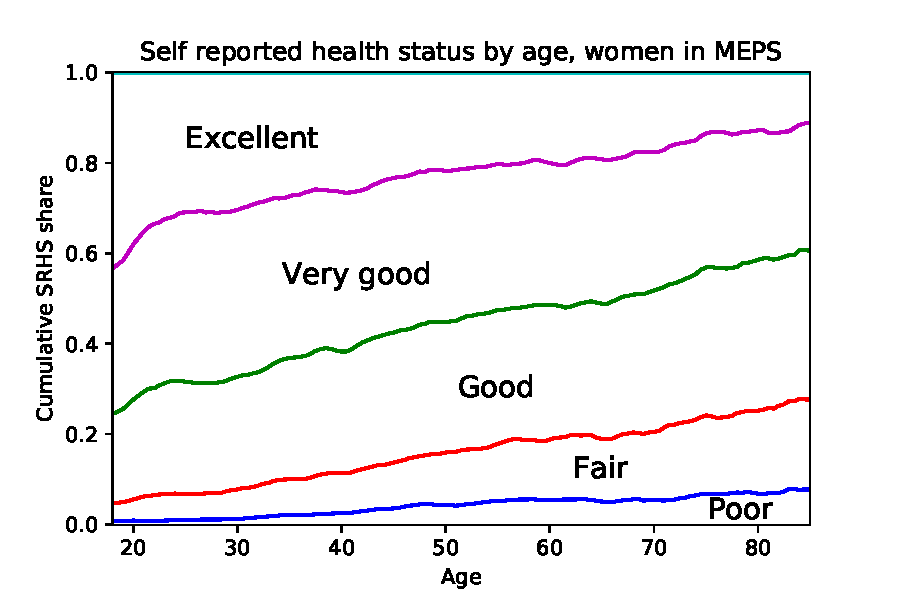
\includegraphics[scale=0.65]{\FigsDir/MEPSover18WomenSRHSbyAgeDataOnly.pdf}
	\caption{Empirical distribution of SRHS by age, women in MEPS. Distance between colored lines represents share of population reporting each category.}\label{fig:SRHSdstnMEPSwomen}
\end{figure}


\begin{figure}[H]
	\centering
	\begin{subfigure}[b]{0.45\textwidth}
		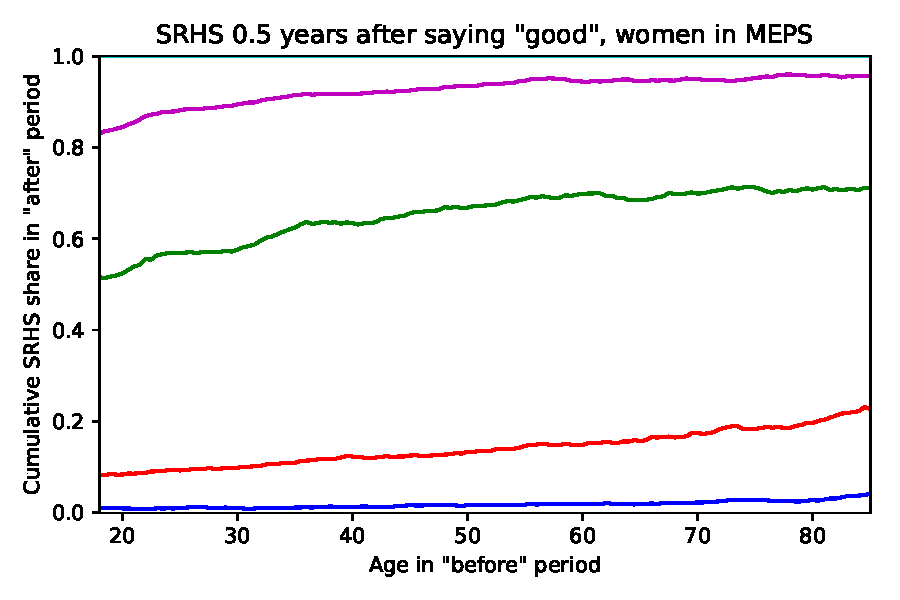
\includegraphics[width=\textwidth]{\FigsDir/MEPSover18WomenTransH3T1naiveNoLeg.pdf}
		\caption{One period ahead}\label{fig:Naive1Ahead}
	\end{subfigure}
	~
	\begin{subfigure}[b]{0.45\textwidth}
		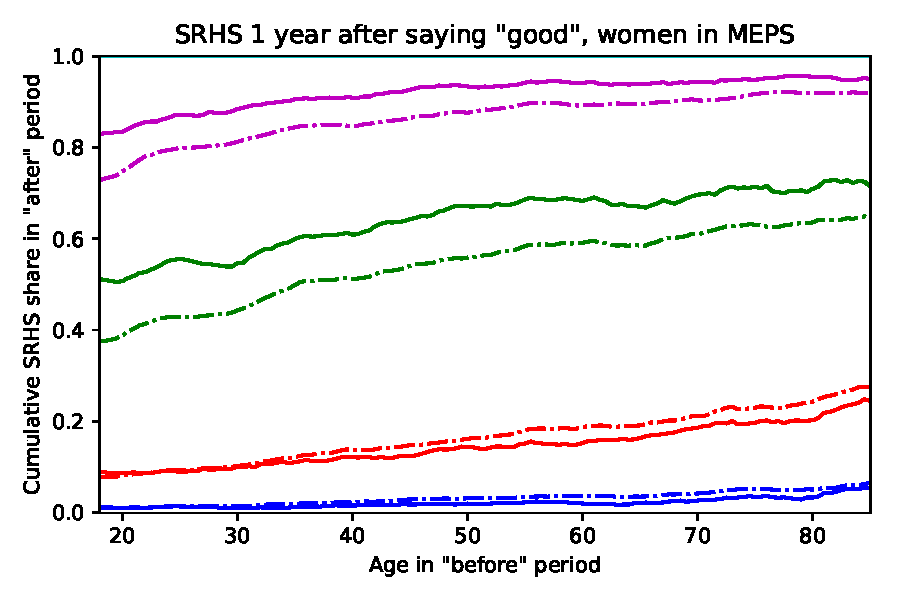
\includegraphics[width=\textwidth]{\FigsDir/MEPSover18WomenTransH3T2naiveNoLeg.pdf}
		\caption{Two periods ahead}\label{fig:Naive2Ahead}
	\end{subfigure}
	
	\begin{subfigure}[b]{0.45\textwidth}
		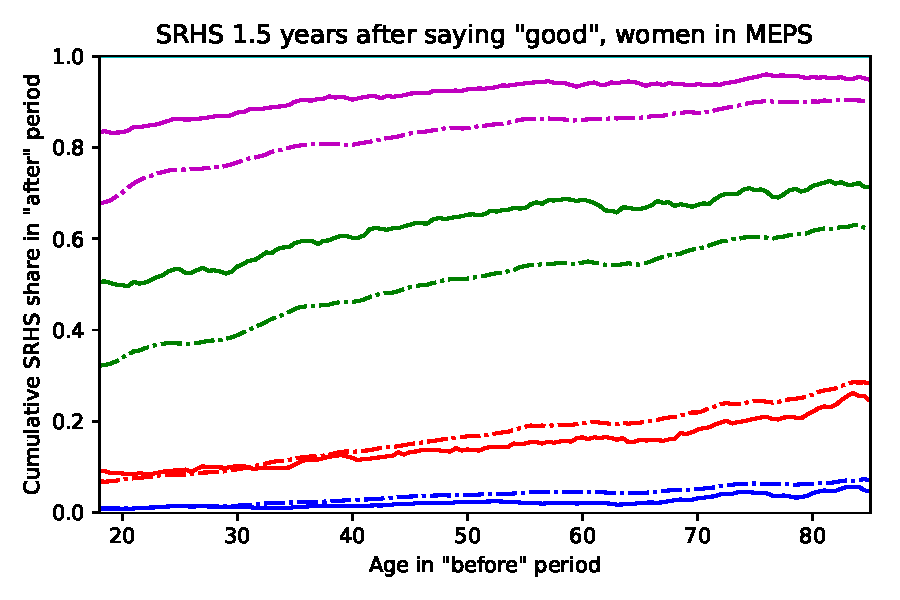
\includegraphics[width=\textwidth]{\FigsDir/MEPSover18WomenTransH3T3naiveNoLeg.pdf}
		\caption{Three periods ahead}\label{fig:Naive3Ahead}
	\end{subfigure}
	~
	\begin{subfigure}[b]{0.45\textwidth}
		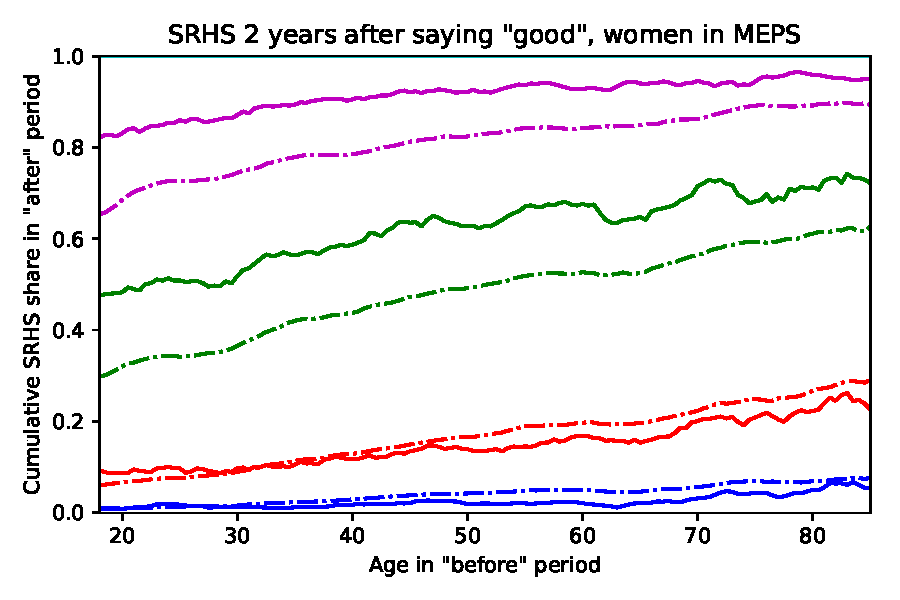
\includegraphics[width=\textwidth]{\FigsDir/MEPSover18WomenTransH3T4naiveNoLeg.pdf}
		\caption{Four periods ahead}\label{fig:Naive4AheadGood}
	\end{subfigure}
	\caption{Cumulative distribution of SRHS by age conditional on reporting ``good'' health in the baseline period in the MEPS data (solid) vs under naive dynamics (dash-dot).  Distribution from naive dynamics exactly matches the data one period ahead (by definition), but strongly deviates from empirical distribution when projected further in the future.}\label{fig:NaiveTransGood}
\end{figure}


\newpage


\begin{figure}[H]
	\centering
	\begin{subfigure}[b]{0.45\textwidth}
		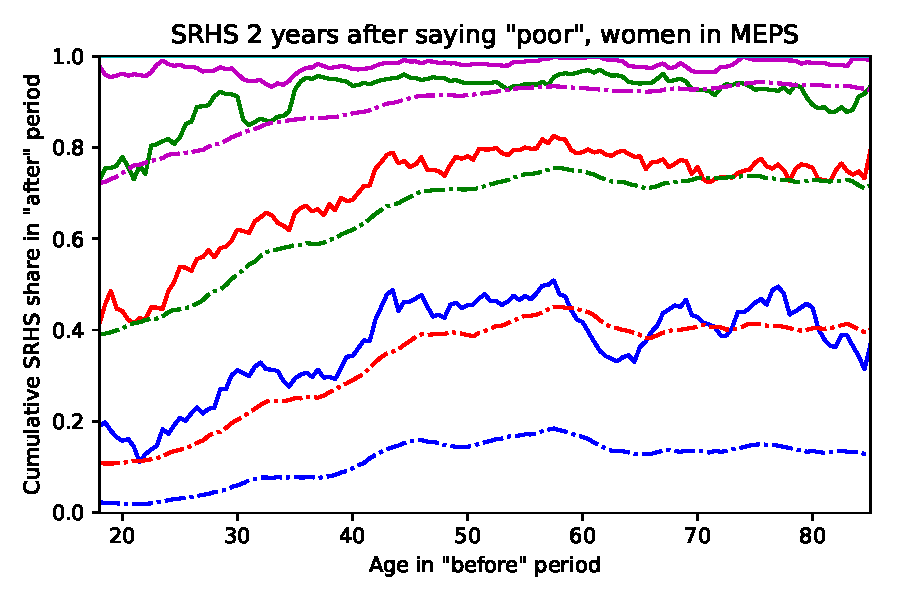
\includegraphics[width=\textwidth]{\FigsDir/MEPSover18WomenTransH1T4naiveNoLeg.pdf}
		\caption{Poor health at baseline}\label{fig:Naive4AheadPoor}
	\end{subfigure}
	~
	\begin{subfigure}[b]{0.45\textwidth}
		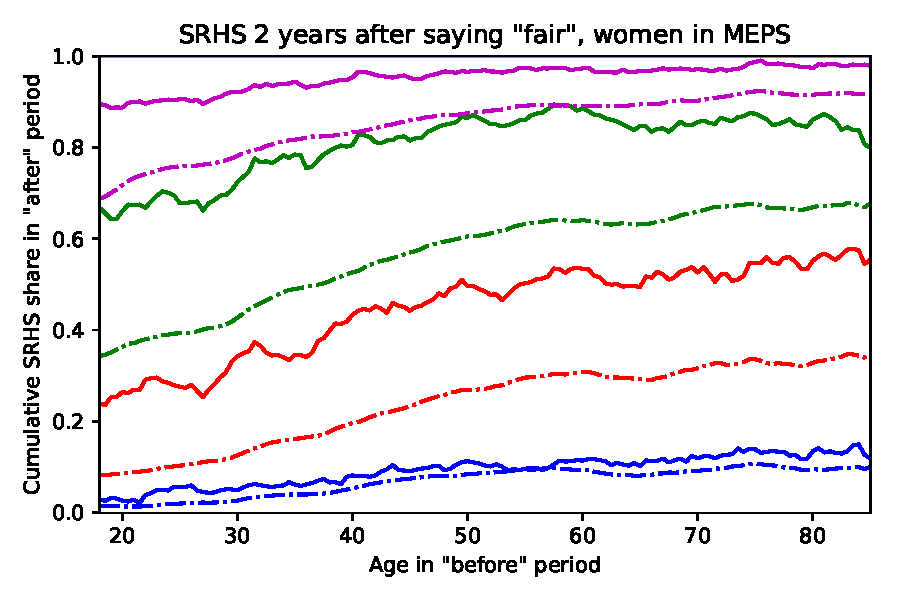
\includegraphics[width=\textwidth]{\FigsDir/MEPSover18WomenTransH2T4naiveNoLeg.pdf}
		\caption{Fair health at baseline}\label{fig:Naive4AheadFair}
	\end{subfigure}
	
	\begin{subfigure}[b]{0.45\textwidth}
		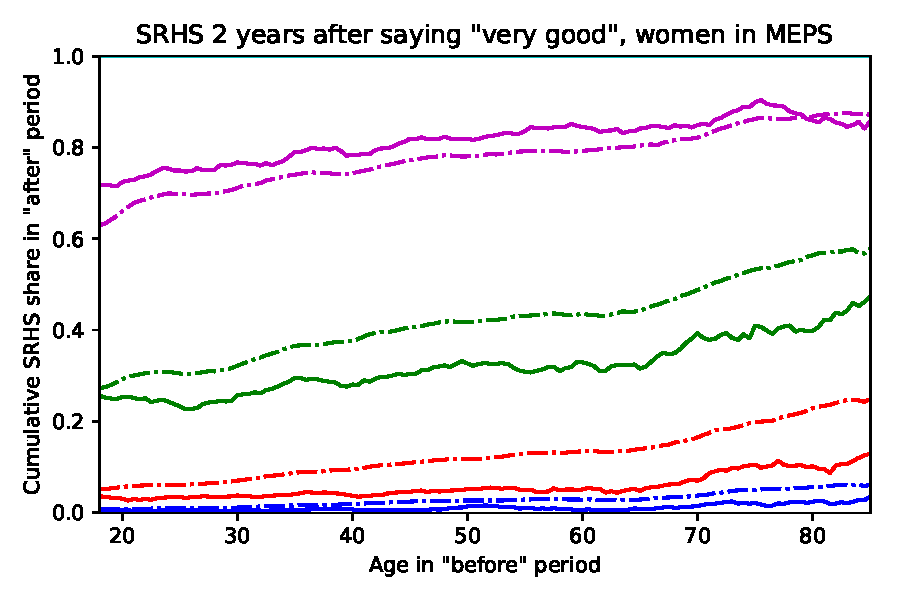
\includegraphics[width=\textwidth]{\FigsDir/MEPSover18WomenTransH4T4naiveNoLeg.pdf}
		\caption{Very good health at baseline}\label{fig:Naive4AheadVeryGood}
	\end{subfigure}
	~
	\begin{subfigure}[b]{0.45\textwidth}
		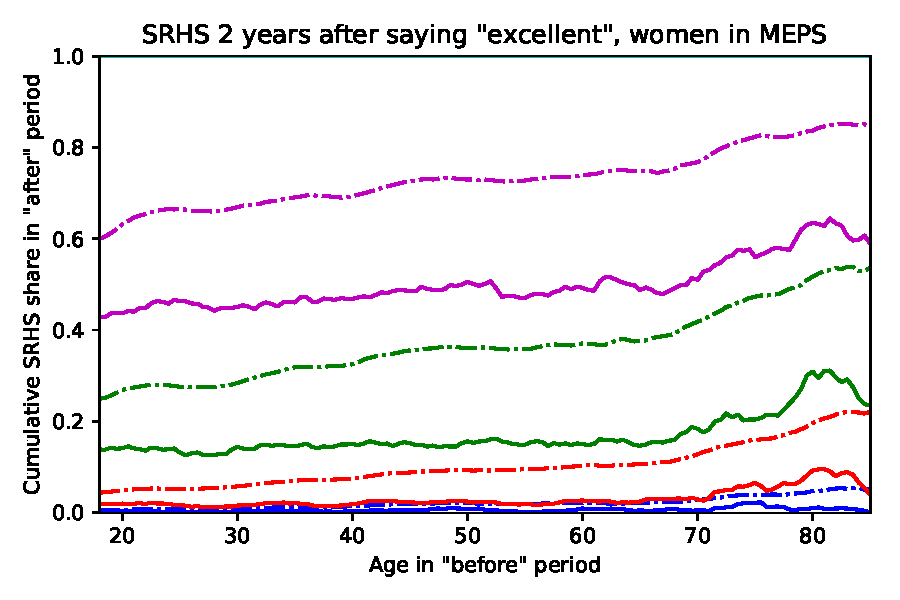
\includegraphics[width=\textwidth]{\FigsDir/MEPSover18WomenTransH5T4naiveNoLeg.pdf}
		\caption{Excellent health at baseline}\label{fig:Naive4AheadExcellent}
	\end{subfigure}
	\caption{Cumulative distribution of SRHS by age after the baseline period in the MEPS data (solid) vs under naive dynamics (dash-dot)}\label{fig:NaiveTrans4Ahead}
\end{figure}


\begin{figure}[H]
	\centering
	\begin{subfigure}[b]{0.48\textwidth}
		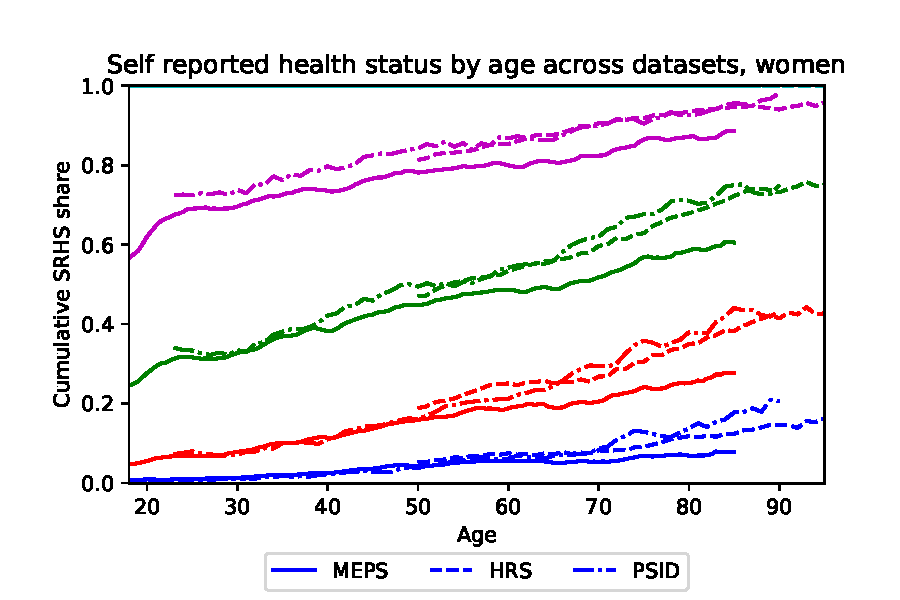
\includegraphics[width=\textwidth]{\FigsDir/CrossDataSRHSaWomen.pdf}
		\caption{MEPS vs HRS vs PSID}\label{fig:SRHScompareA}
	\end{subfigure}
    ~
    \begin{subfigure}[b]{0.48\textwidth}
    	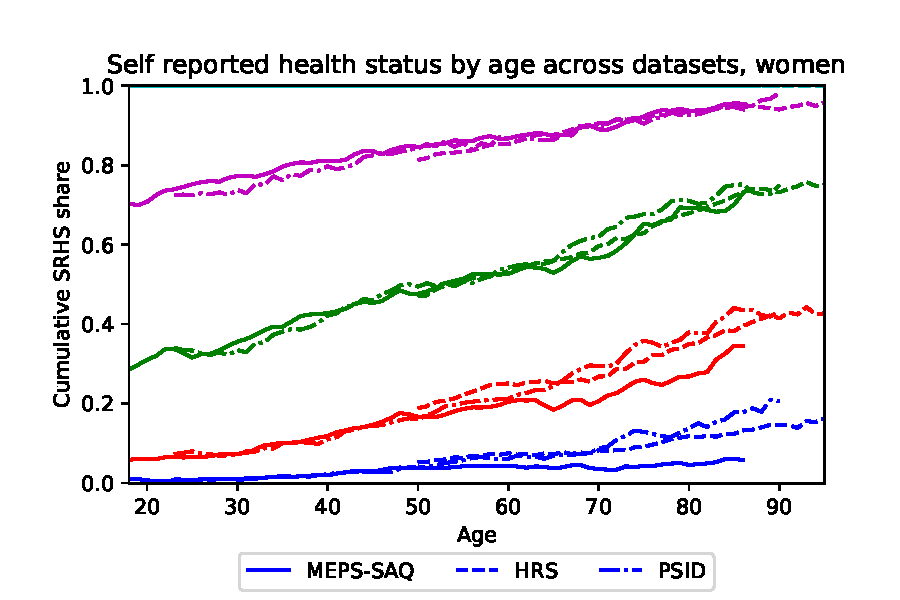
\includegraphics[width=\textwidth]{\FigsDir/CrossDataSRHSbWomen.pdf}
    	\caption{MEPS-SAQ vs HRS vs PSID}\label{fig:SRHScompareB}
    \end{subfigure}
	\caption{Distribution of SRHS by age for women across datasets. Standard MEPS deviates from distribution in HRS and PSID, possibly due to question wording.  MEPS-SAQ more closely matches, but has more selection bias for those in poor health.}\label{fig:SRHScompare}
\end{figure}


\newpage

\begin{figure}[H]
	\centering
	\begin{subfigure}[b]{0.48\textwidth}
	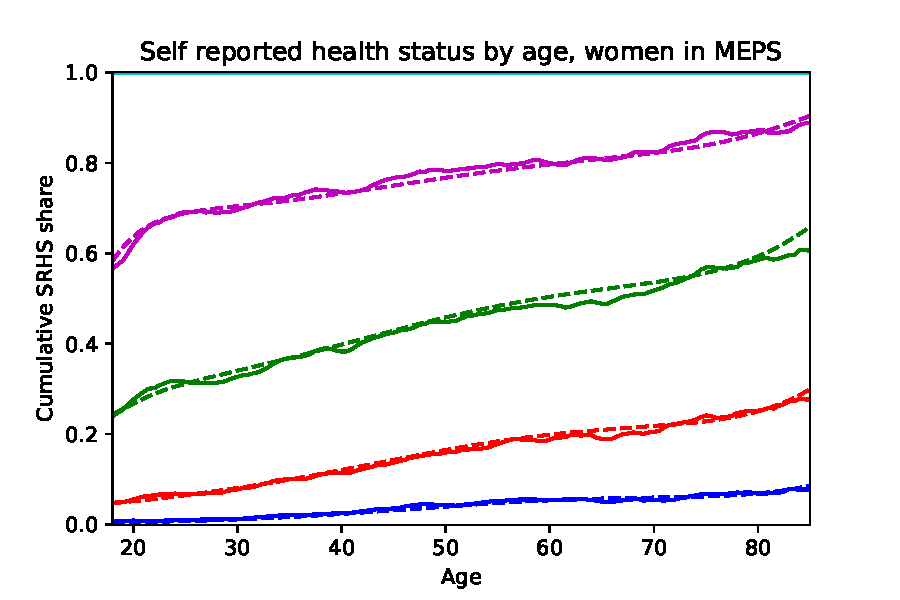
\includegraphics[width=\textwidth]{\FigsDir/MEPSover18WomenSRHSbyAge.pdf}
	\caption{MEPS women}\label{fig:MEPSwomenSRHSfit}
	\end{subfigure}
    ~
    \begin{subfigure}[b]{0.48\textwidth}
    	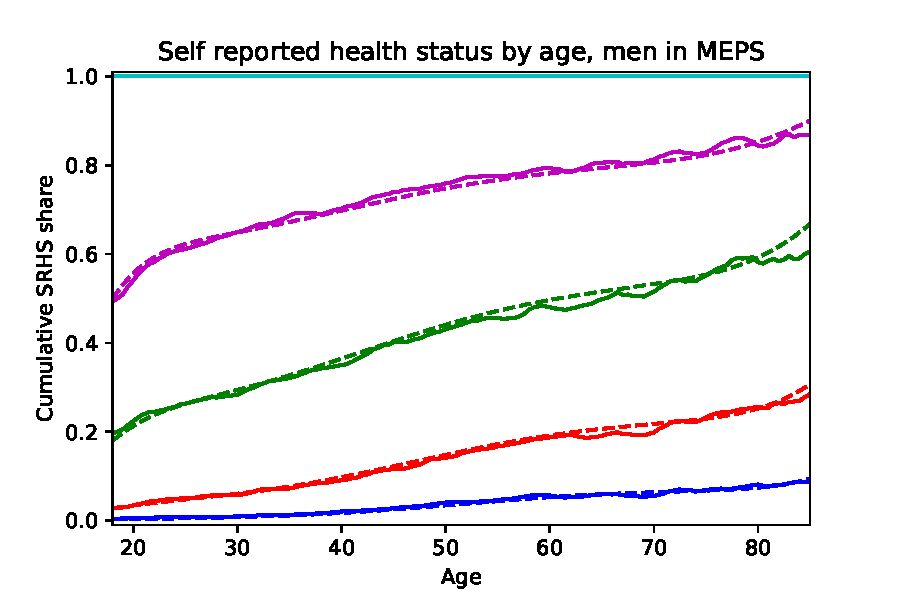
\includegraphics[width=\textwidth]{\FigsDir/MEPSover18MenSRHSbyAge.pdf}
    	\caption{MEPS men}\label{fig:MEPSmenSRHSfit}
    \end{subfigure}
    \caption{Distribution of SRHS by age, MEPS data (solid) vs estimated model (dashed)}\label{fig:SRHSfitMEPS}
\end{figure}


\begin{figure}[H]
	\centering
	\begin{subfigure}[b]{0.48\textwidth}
		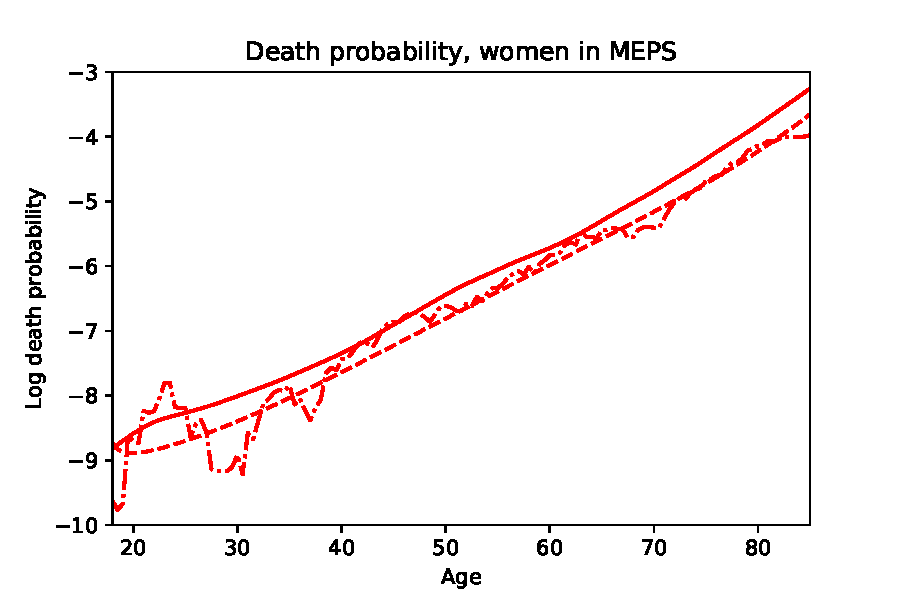
\includegraphics[width=\textwidth]{\FigsDir/MEPSover18WomenMortByAge.pdf}
		\caption{MEPS women}\label{fig:MEPSwomenMortFit}
	\end{subfigure}
	~
	\centering
	\begin{subfigure}[b]{0.48\textwidth}
		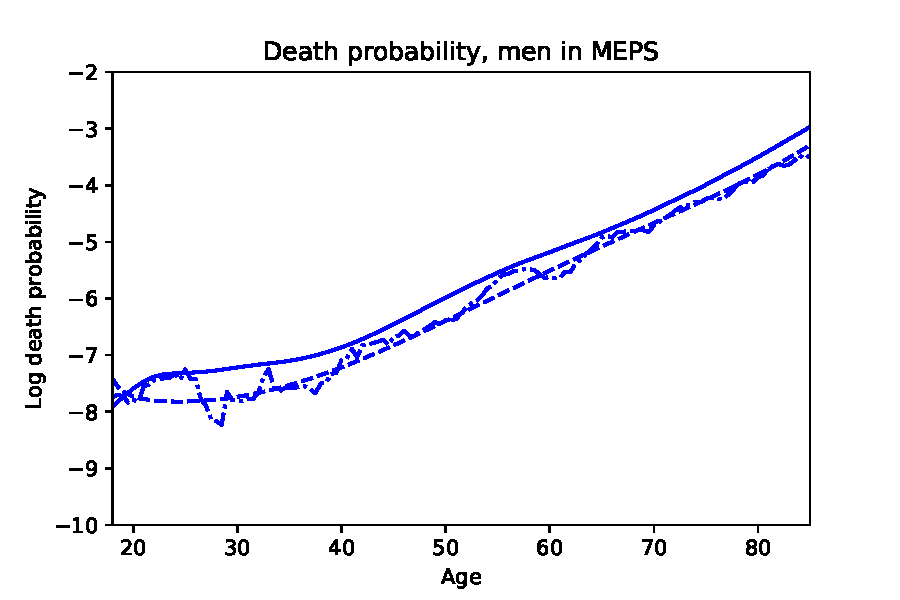
\includegraphics[width=\textwidth]{\FigsDir/MEPSover18MenMortByAge.pdf}
		\caption{MEPS men}\label{fig:MEPSmenMortFit}
	\end{subfigure}
	\caption{Mortality by age, SSA table (solid) vs MEPS data (dash-dot) vs estimated model} \label{fig:MortFitMEPS}
\end{figure}


\begin{figure}[H]
	\centering
	\begin{subfigure}[b]{0.48\textwidth}
		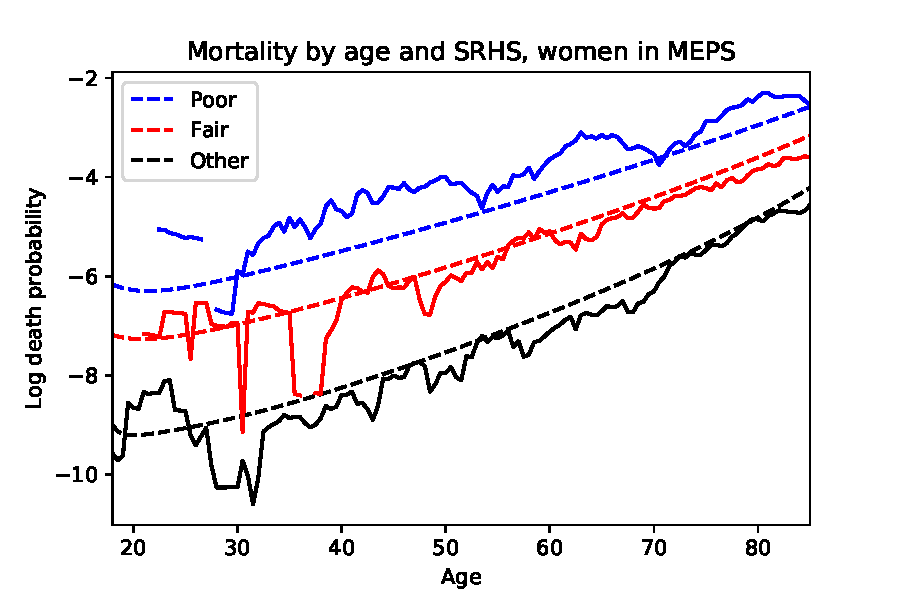
\includegraphics[width=\textwidth]{\FigsDir/MEPSover18WomenMortByAgeHealth.pdf}
		\caption{MEPS women}\label{fig:MEPSwomenMortHealthFit}
	\end{subfigure}
	~
	\centering
	\begin{subfigure}[b]{0.48\textwidth}
		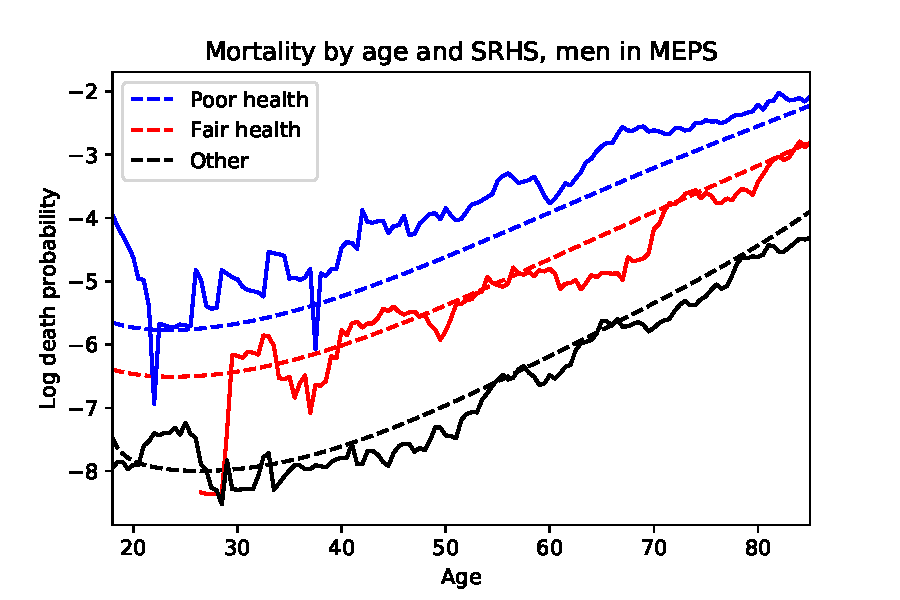
\includegraphics[width=\textwidth]{\FigsDir/MEPSover18MenMortByAgeHealth.pdf}
		\caption{MEPS men}\label{fig:MEPSmenMortHealthFit}
	\end{subfigure}
	\caption{Mortality by age and health, MEPS data (solid) vs estimated model (dashed)} \label{fig:MortFitByHealthMEPS}
\end{figure}

\newpage

\begin{figure}[H]
	\centering
	\begin{subfigure}[b]{0.45\textwidth}
		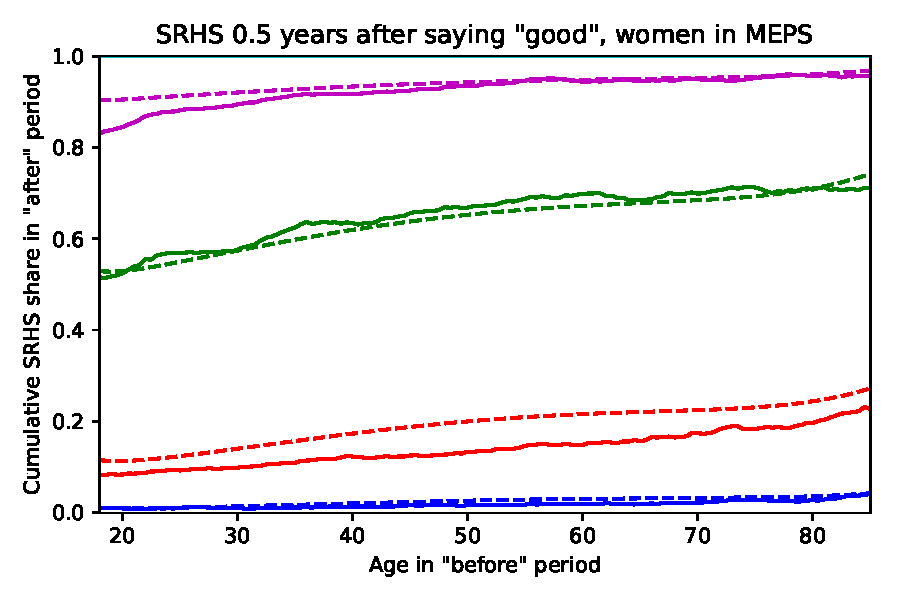
\includegraphics[width=\textwidth]{\FigsDir/MEPSover18WomenTransH3T1modelNoLeg.pdf}
		\caption{One period ahead}\label{fig:Model1Ahead}
	\end{subfigure}
	~
	\begin{subfigure}[b]{0.45\textwidth}
		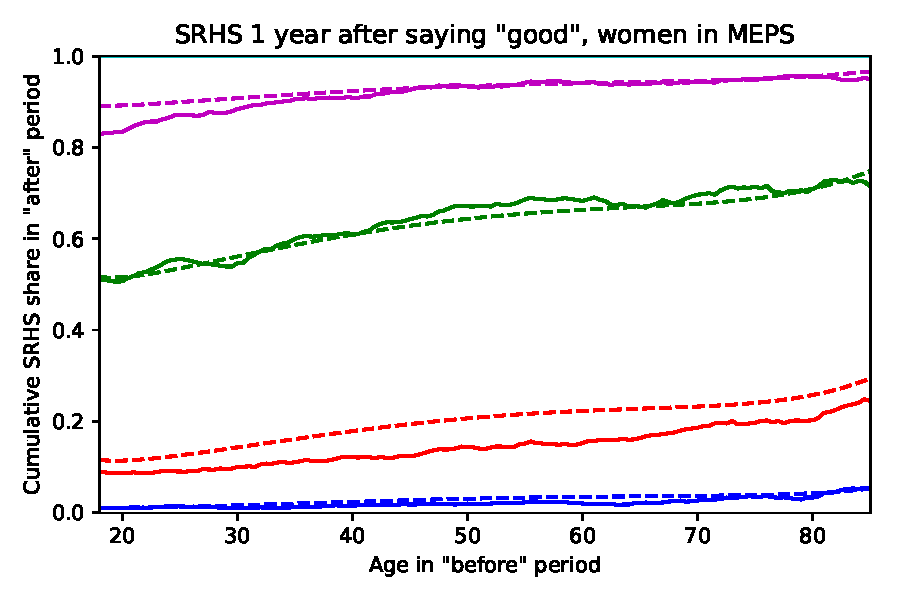
\includegraphics[width=\textwidth]{\FigsDir/MEPSover18WomenTransH3T2modelNoLeg.pdf}
		\caption{Two periods ahead}\label{fig:Model2Ahead}
	\end{subfigure}
	
	\begin{subfigure}[b]{0.45\textwidth}
		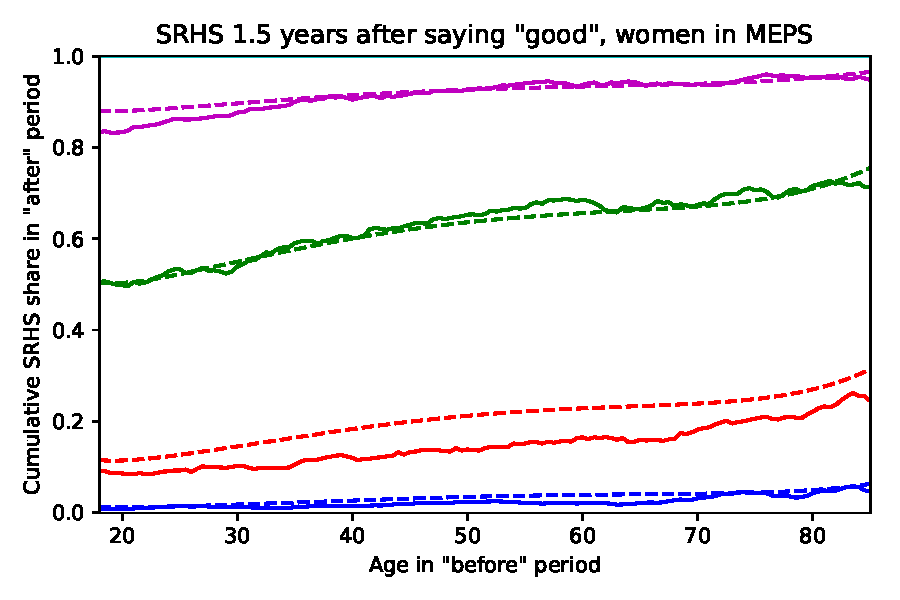
\includegraphics[width=\textwidth]{\FigsDir/MEPSover18WomenTransH3T3modelNoLeg.pdf}
		\caption{Three periods ahead}\label{fig:Model3Ahead}
	\end{subfigure}
	~
	\begin{subfigure}[b]{0.45\textwidth}
		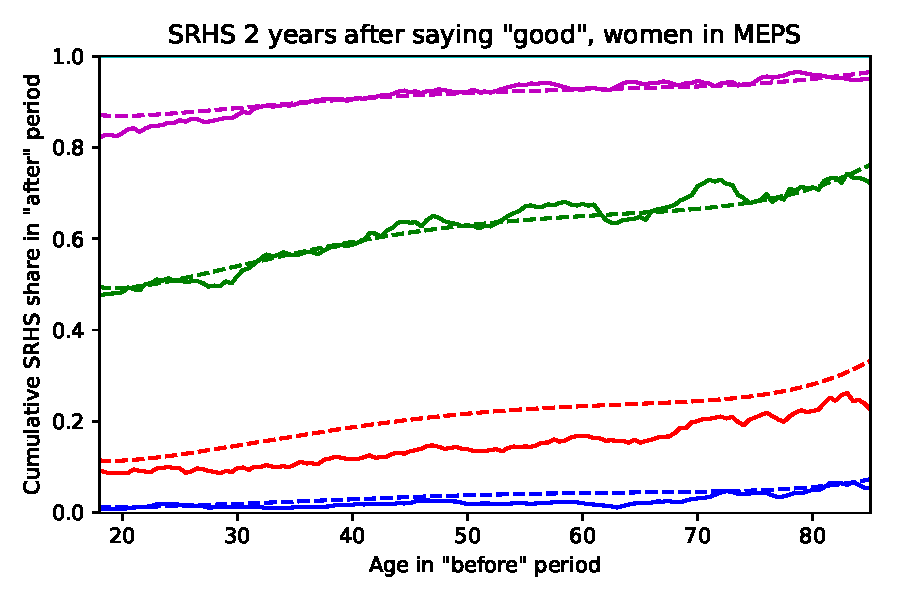
\includegraphics[width=\textwidth]{\FigsDir/MEPSover18WomenTransH3T4modelNoLeg.pdf}
		\caption{Four periods ahead}\label{fig:Model4AheadGood}
	\end{subfigure}
	\caption{Cumulative distribution of SRHS by age conditional on reporting ``good'' health in the baseline period in the MEPS data (solid) vs estimated model (dashed)}\label{fig:ModelTransMEPSgood}
\end{figure}

\begin{figure}[H]
	\centering
	\begin{subfigure}[b]{0.48\textwidth}
		\includegraphics[width=\textwidth]{\FigsDir/MEPSover18WomenSameSRHS.pdf}
		\caption{MEPS women}
	\end{subfigure}
	~
	\begin{subfigure}[b]{0.48\textwidth}
		\includegraphics[width=\textwidth]{\FigsDir/MEPSover18MenSameSRHS.pdf}
		\caption{MEPS men}
	\end{subfigure}
	\caption{Proportion of respondents who report the same SRHS in all five waves of MEPS (balanced panel) vs estimated model.  Model under-predicts this feature by about 7\%.}\label{fig:MEPSsameSRHS}
\end{figure}

\newpage


\begin{figure}[H]
	\centering
	\begin{subfigure}[b]{0.45\textwidth}
		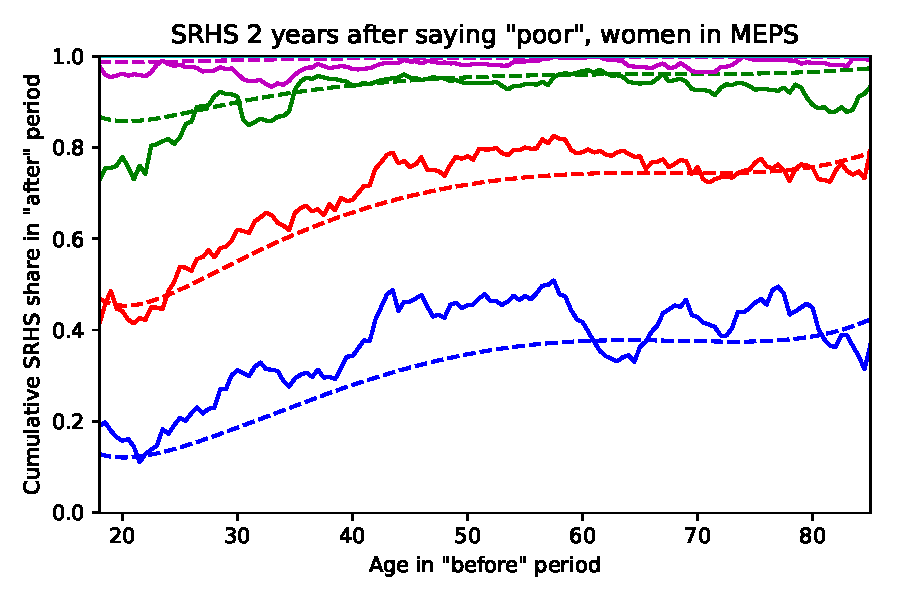
\includegraphics[width=\textwidth]{\FigsDir/MEPSover18WomenTransH1T4modelNoLeg.pdf}
		\caption{Poor health at baseline}\label{fig:Model4AheadPoor}
	\end{subfigure}
	~
	\begin{subfigure}[b]{0.45\textwidth}
		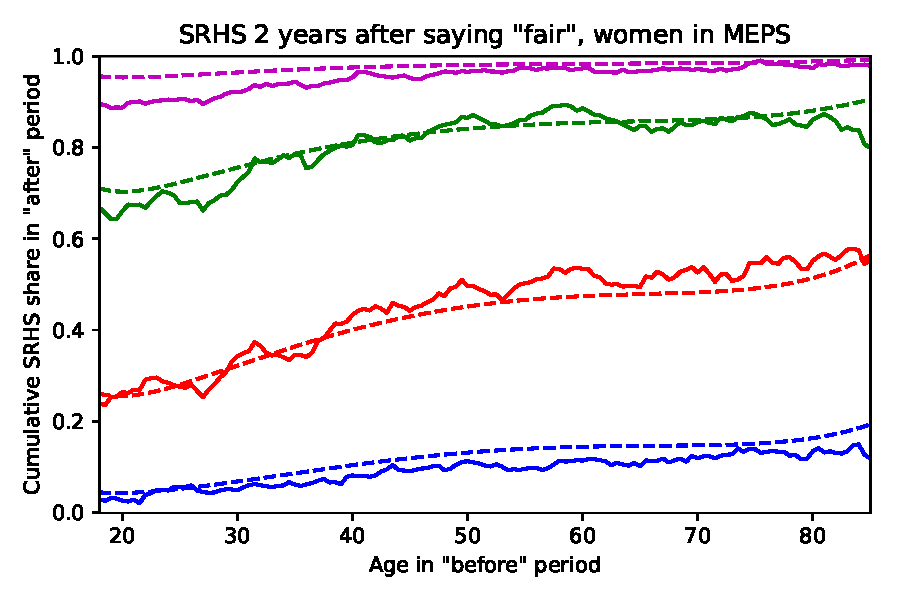
\includegraphics[width=\textwidth]{\FigsDir/MEPSover18WomenTransH2T4modelNoLeg.pdf}
		\caption{Fair health at baseline}\label{fig:Model4AheadFair}
	\end{subfigure}
	
	\begin{subfigure}[b]{0.45\textwidth}
		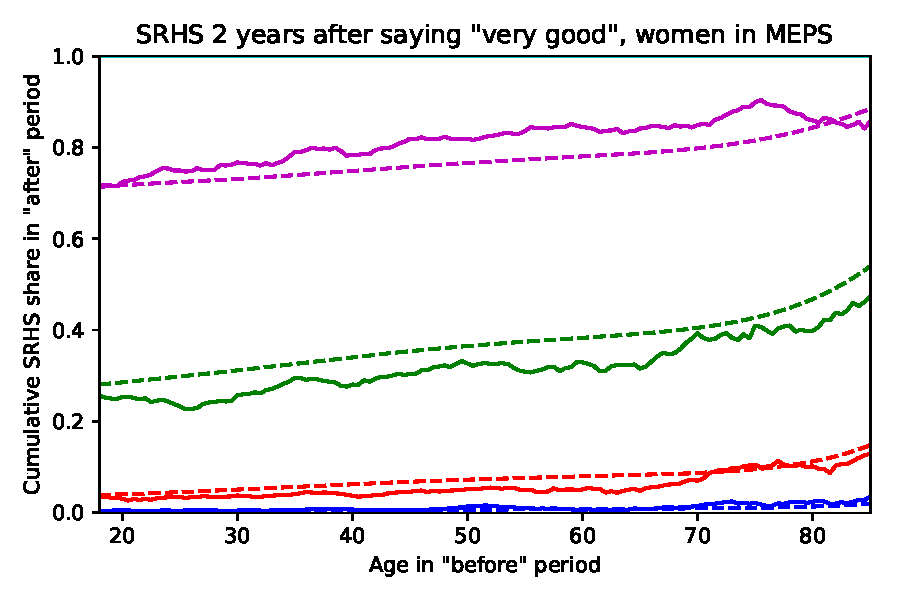
\includegraphics[width=\textwidth]{\FigsDir/MEPSover18WomenTransH4T4modelNoLeg.pdf}
		\caption{Very good health at baseline}\label{fig:Model4AheadVeryGood}
	\end{subfigure}
	~
	\begin{subfigure}[b]{0.45\textwidth}
		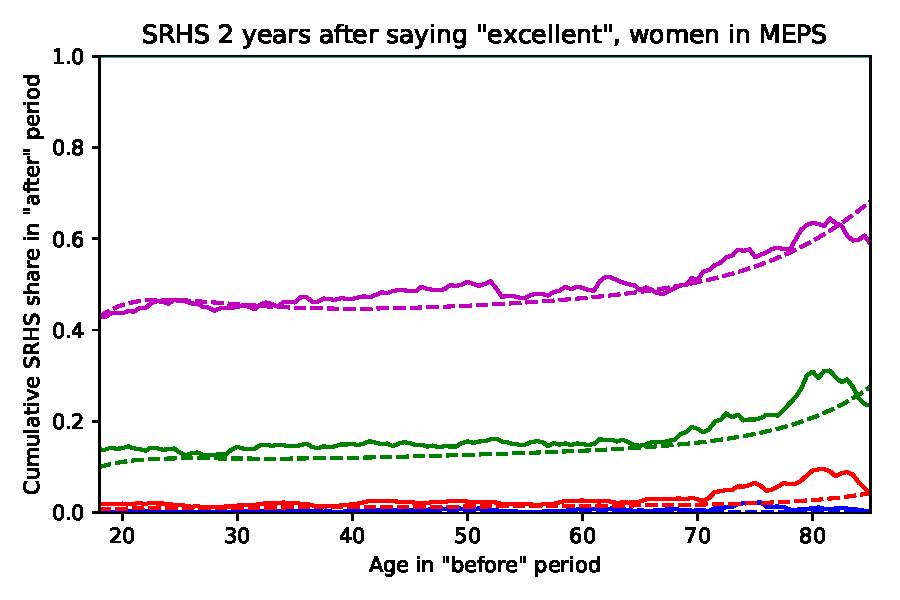
\includegraphics[width=\textwidth]{\FigsDir/MEPSover18WomenTransH5T4modelNoLeg.pdf}
		\caption{Excellent health at baseline}\label{fig:Model4AheadExcellent}
	\end{subfigure}
	\caption{Cumulative distribution of SRHS by age two years after the baseline period in the MEPS data (solid) vs estimated model (dashed)}\label{fig:ModelTransMEPS4ahead}
\end{figure}


\begin{figure}[H]
	\centering
	\begin{subfigure}[b]{0.48\textwidth}
		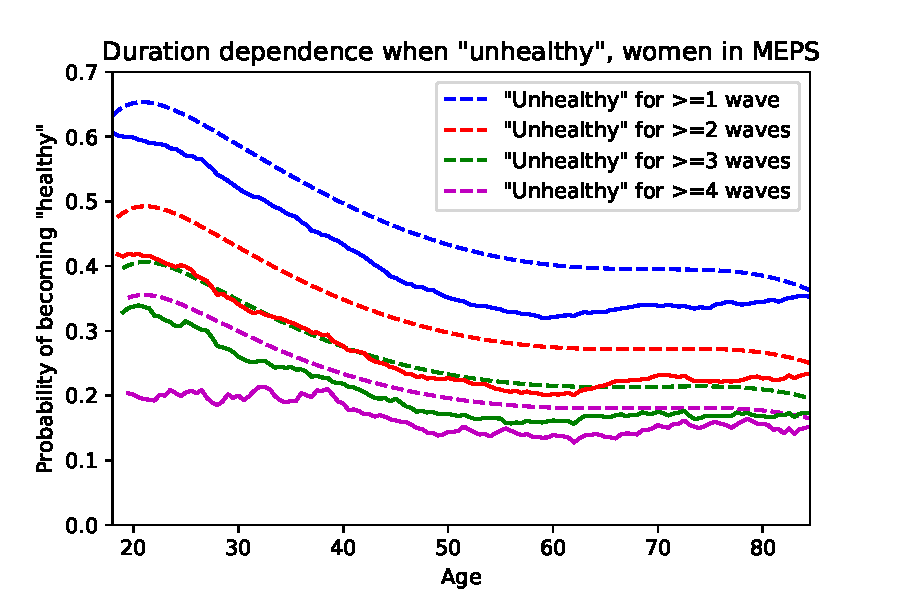
\includegraphics[width=\textwidth]{\FigsDir/MEPSover18WomenDurDepT4B2G.pdf}
		\caption{Duration dependence of bad health}\label{fig:DurDepMEPSwomenB2G}
	\end{subfigure}
	~
	\begin{subfigure}[b]{0.48\textwidth}
		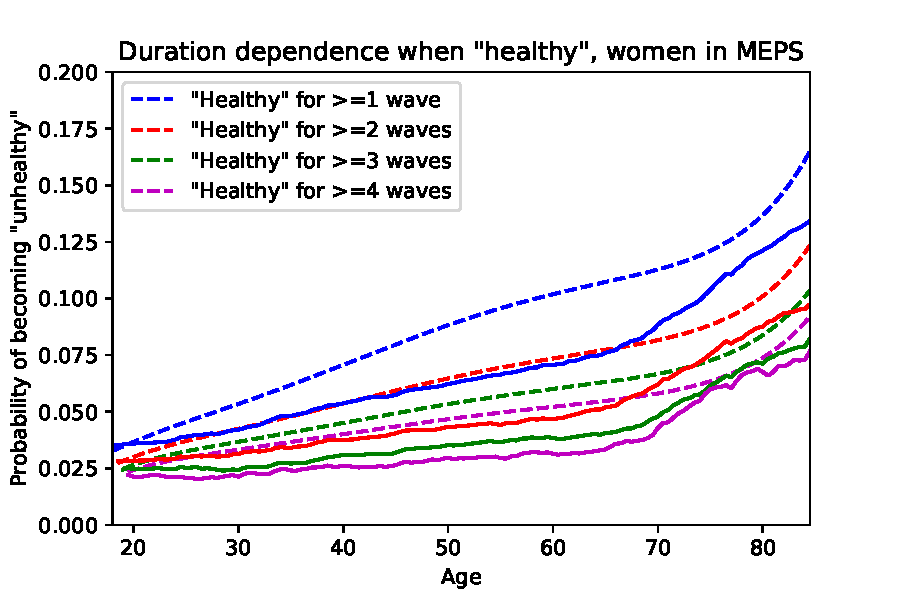
\includegraphics[width=\textwidth]{\FigsDir/MEPSover18WomenDurDepT4G2B.pdf}
		\caption{Duration dependence of good health}\label{fig:DurDepMEPSwomenG2B}
	\end{subfigure}
\caption{Duration dependence of being ``healthy'' and ``unhealthy'' for women in MEPS data (solid) vs estimated model (dashed).}\label{fig:DurDepMEPSwomen}
\end{figure}

\newpage



\begin{figure}[H]
	\centering
	\begin{subfigure}[b]{0.48\textwidth}
		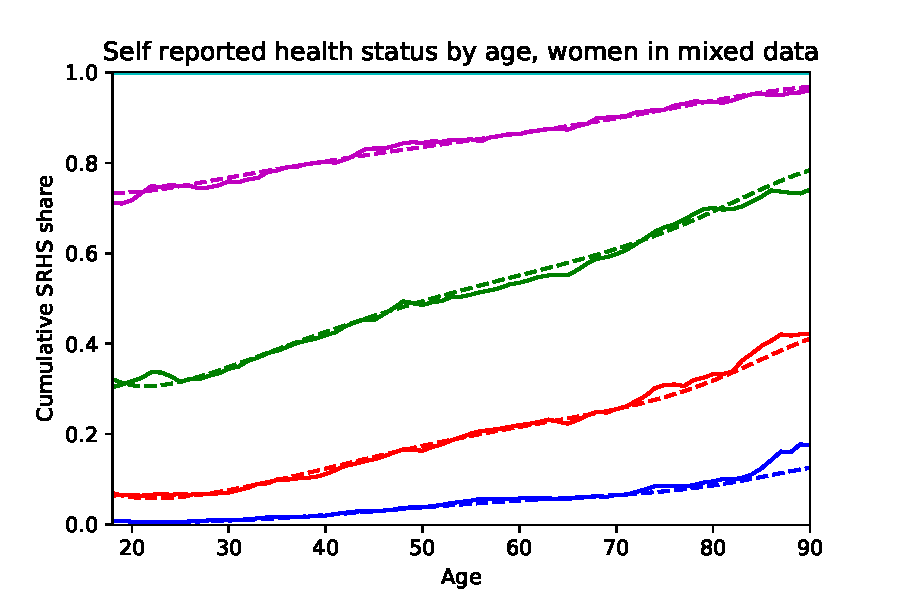
\includegraphics[width=\textwidth]{\FigsDir/CrossDataWomenSRHSbyAge.pdf}
		\caption{Mixed data women}\label{fig:MixedWomenSRHSfit}
	\end{subfigure}
	~
	\begin{subfigure}[b]{0.48\textwidth}
		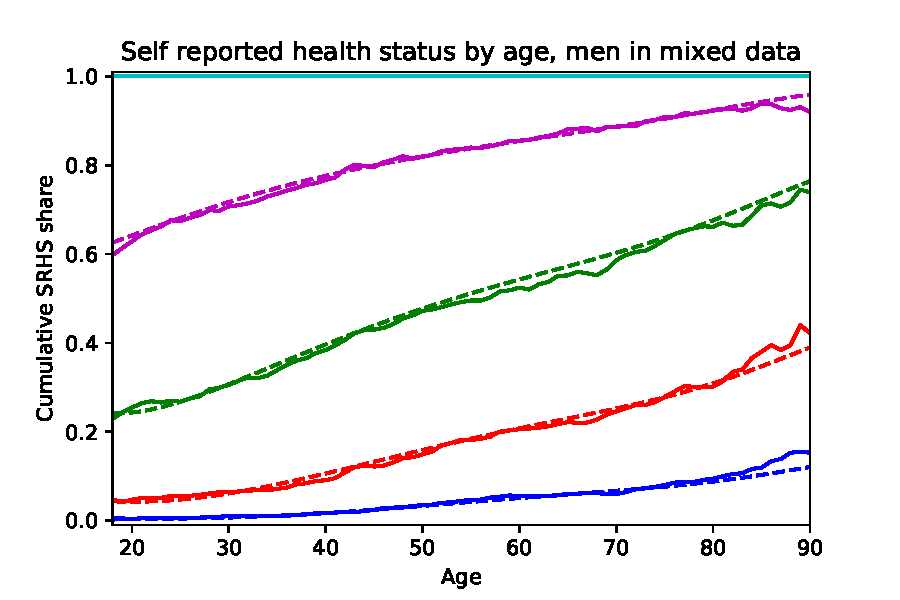
\includegraphics[width=\textwidth]{\FigsDir/CrossDataMenSRHSbyAge.pdf}
		\caption{Mixed data men}\label{fig:MixedMenSRHSfit}
	\end{subfigure}
	\caption{Distribution of SRHS by age, mixed data (solid) vs estimated model (dashed)}\label{fig:SRHSfitMixed}
\end{figure}


\begin{figure}[H]
	\centering
	\begin{subfigure}[b]{0.48\textwidth}
		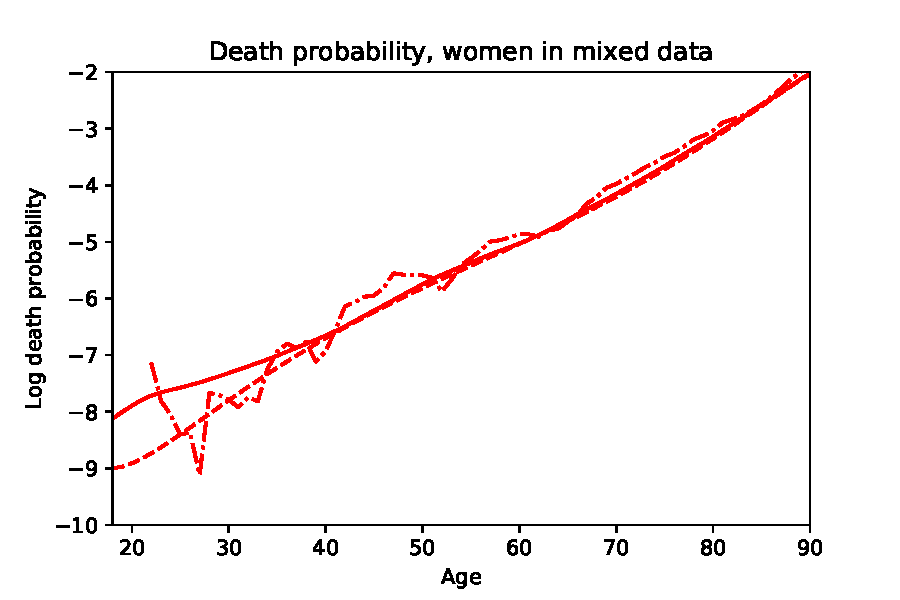
\includegraphics[width=\textwidth]{\FigsDir/CrossDataWomenMortByAge.pdf}
		\caption{Mixed data women}\label{fig:MixedWomenMortFit}
	\end{subfigure}
	~
	\centering
	\begin{subfigure}[b]{0.48\textwidth}
		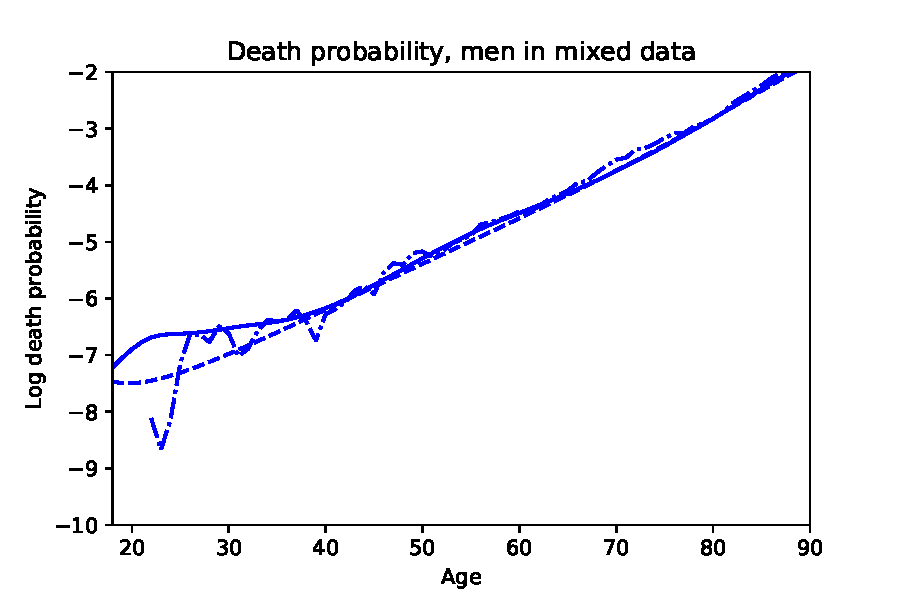
\includegraphics[width=\textwidth]{\FigsDir/CrossDataMenMortByAge.pdf}
		\caption{Mixed data men}\label{fig:MixedMenMortFit}
	\end{subfigure}
	\caption{Mortality by age, SSA table (solid) vs mixed data (dash-dot) vs estimated model} \label{fig:MortFitMixed}
\end{figure}


\begin{figure}[H]
	\centering
	\begin{subfigure}[b]{0.48\textwidth}
		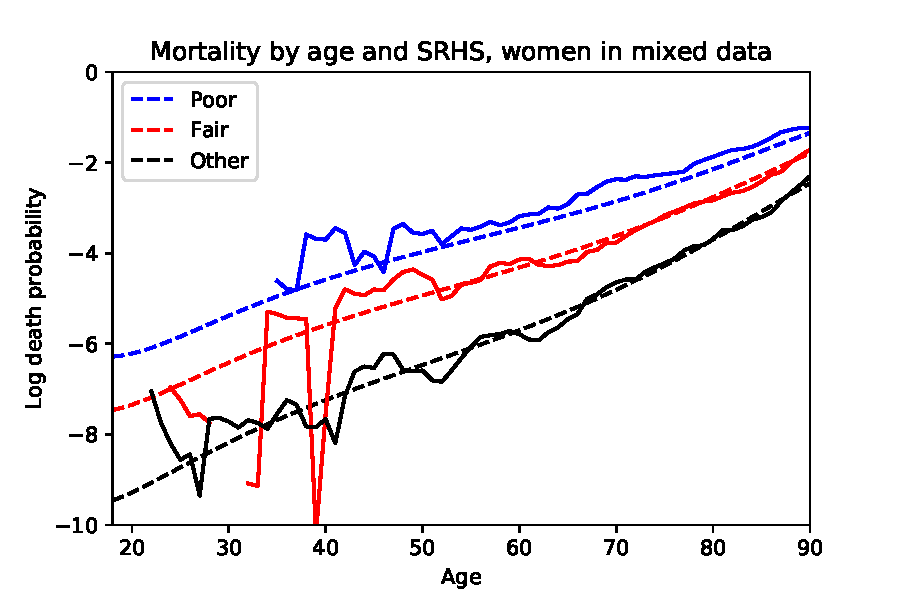
\includegraphics[width=\textwidth]{\FigsDir/CrossDataWomenMortByAgeHealth.pdf}
		\caption{Mixed data women}\label{fig:MixedWomenMortHealthFit}
	\end{subfigure}
	~
	\centering
	\begin{subfigure}[b]{0.48\textwidth}
		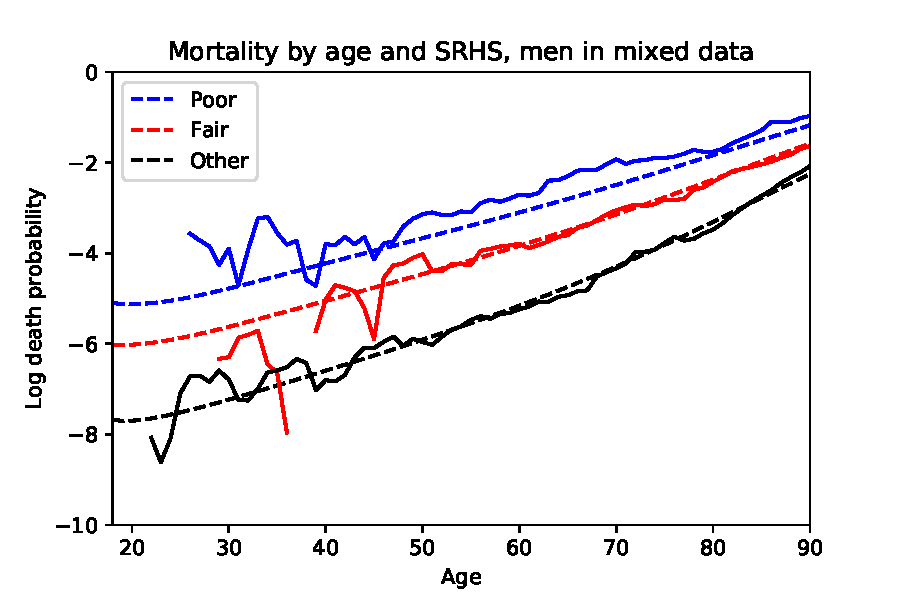
\includegraphics[width=\textwidth]{\FigsDir/CrossDataMenMortByAgeHealth.pdf}
		\caption{Mixed data men}\label{fig:MixedMenMortHealthFit}
	\end{subfigure}
	\caption{Mortality by age and health, mixed data (solid) vs estimated model (dashed)} \label{fig:MortFitByHealthMixed}
\end{figure}

\newpage


\begin{figure}[H]
	\centering
	\begin{subfigure}[b]{0.45\textwidth}
		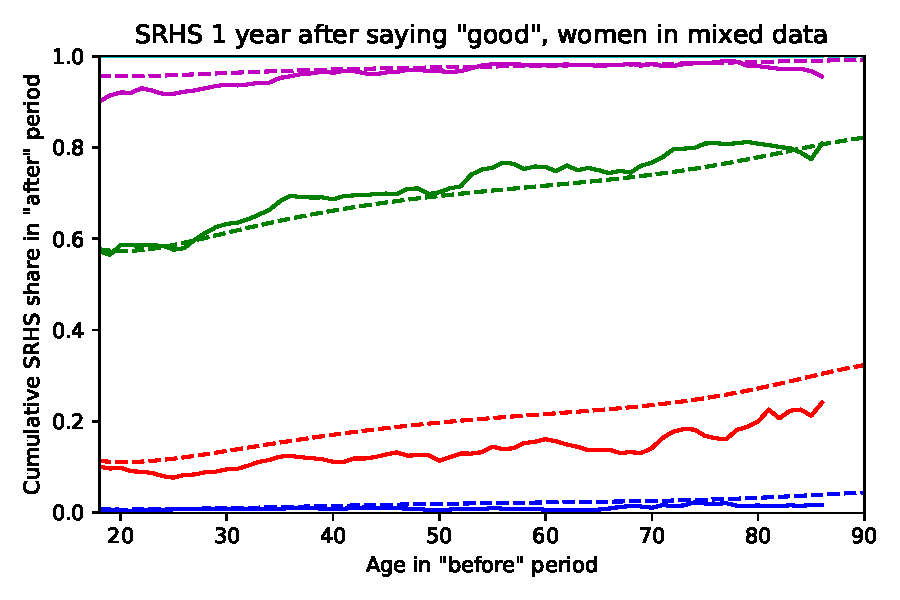
\includegraphics[width=\textwidth]{\FigsDir/CrossDataWomenTransH3T1modelNoLeg.pdf}
		\caption{One year ahead}
	\end{subfigure}
	~
	\begin{subfigure}[b]{0.45\textwidth}
		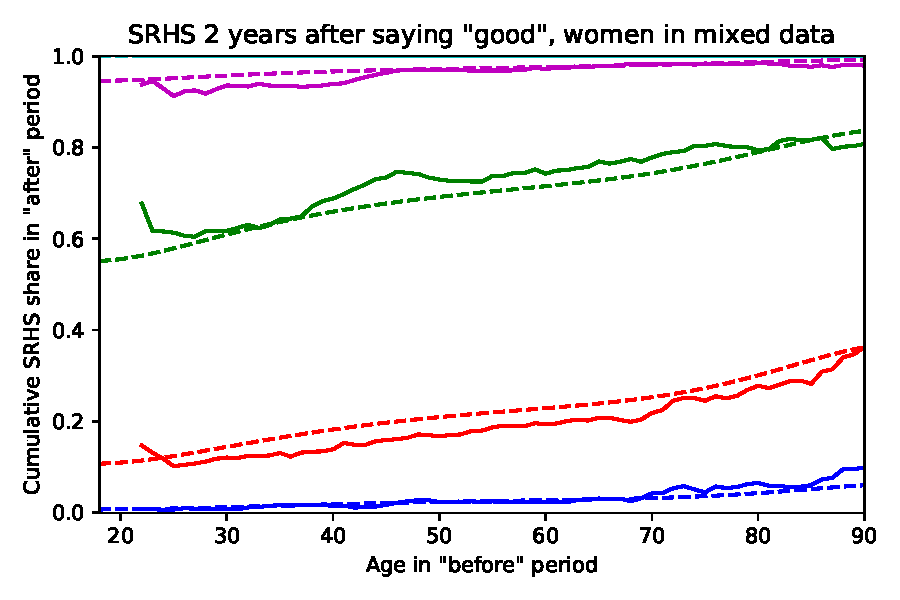
\includegraphics[width=\textwidth]{\FigsDir/CrossDataWomenTransH3T2modelNoLeg.pdf}
		\caption{Two years ahead}
	\end{subfigure}
	
	\begin{subfigure}[b]{0.45\textwidth}
		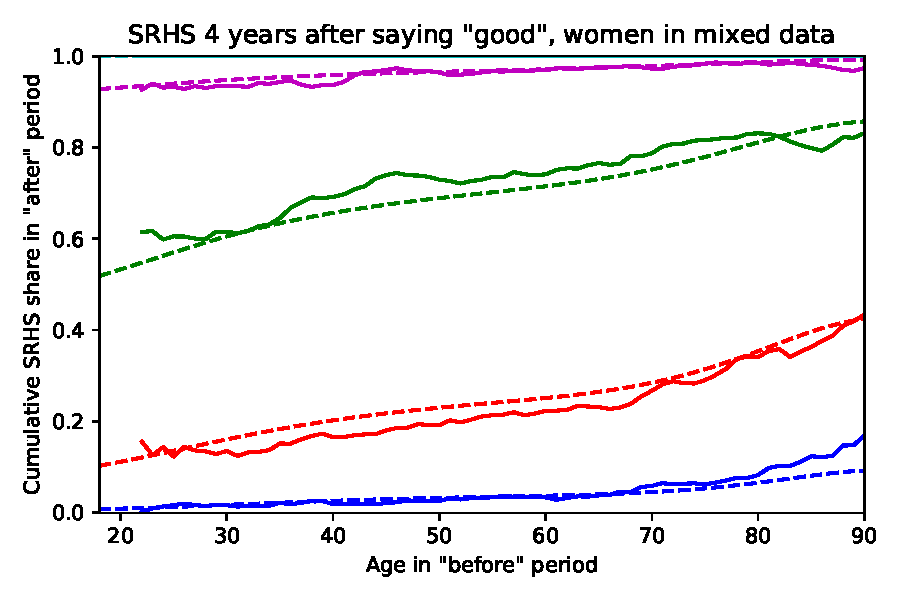
\includegraphics[width=\textwidth]{\FigsDir/CrossDataWomenTransH3T4modelNoLeg.pdf}
		\caption{Four years ahead}
	\end{subfigure}
	~
	\begin{subfigure}[b]{0.45\textwidth}
		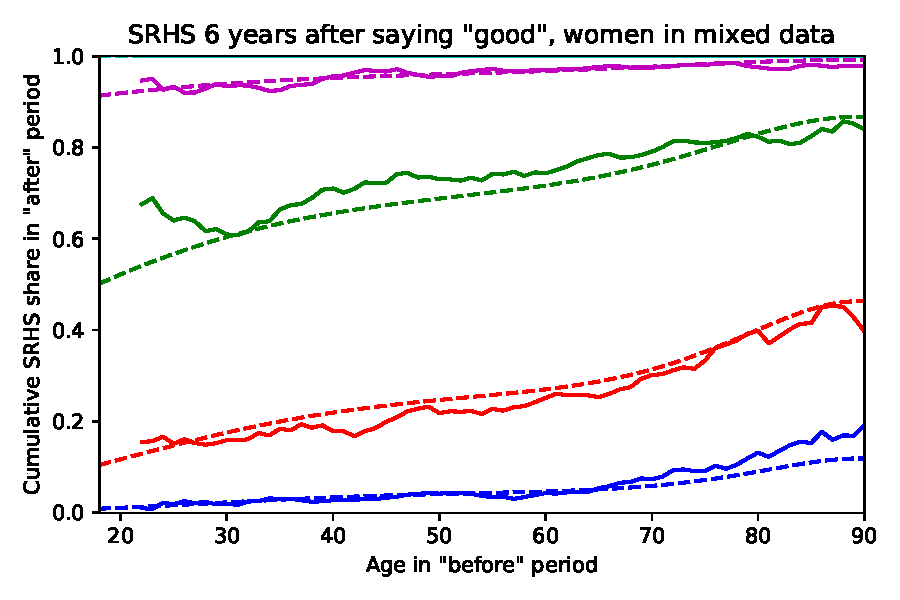
\includegraphics[width=\textwidth]{\FigsDir/CrossDataWomenTransH3T6modelNoLeg.pdf}
		\caption{Six years ahead}
	\end{subfigure}

	\begin{subfigure}[b]{0.45\textwidth}
	    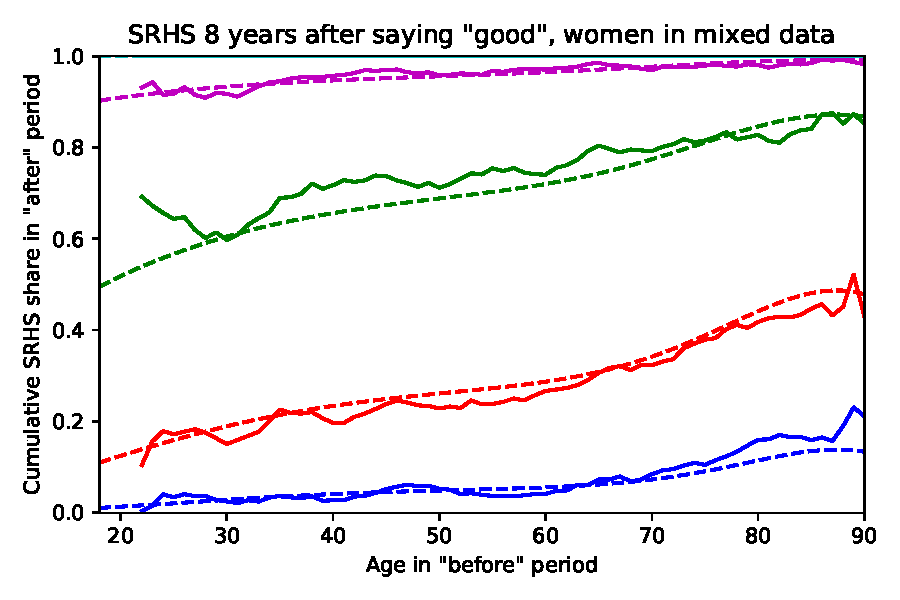
\includegraphics[width=\textwidth]{\FigsDir/CrossDataWomenTransH3T8modelNoLeg.pdf}
	    \caption{Eight years ahead}
    \end{subfigure}
    ~
    \begin{subfigure}[b]{0.45\textwidth}
	    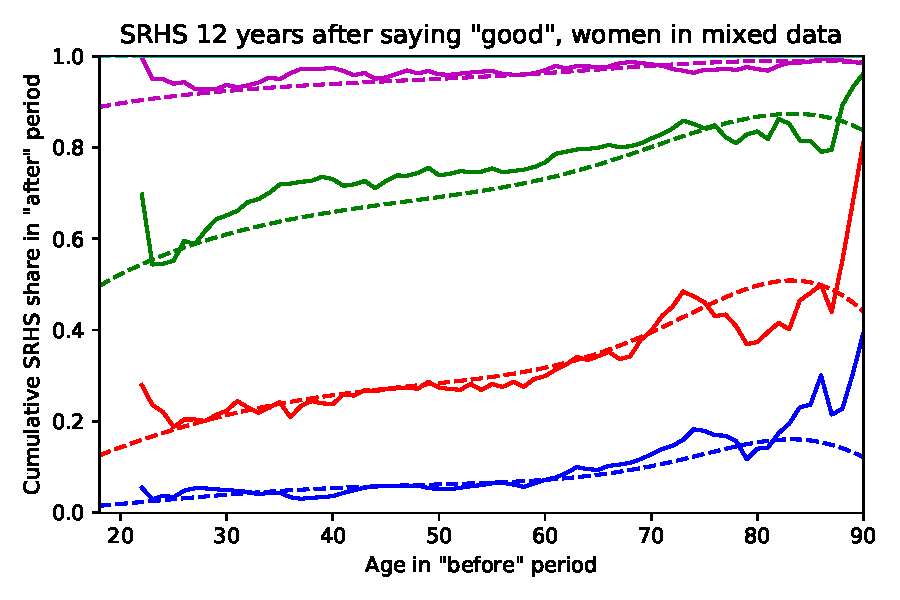
\includegraphics[width=\textwidth]{\FigsDir/CrossDataWomenTransH3T12modelNoLeg.pdf}
	    \caption{Twelve years ahead}
    \end{subfigure}

    \begin{subfigure}[b]{0.45\textwidth}
	    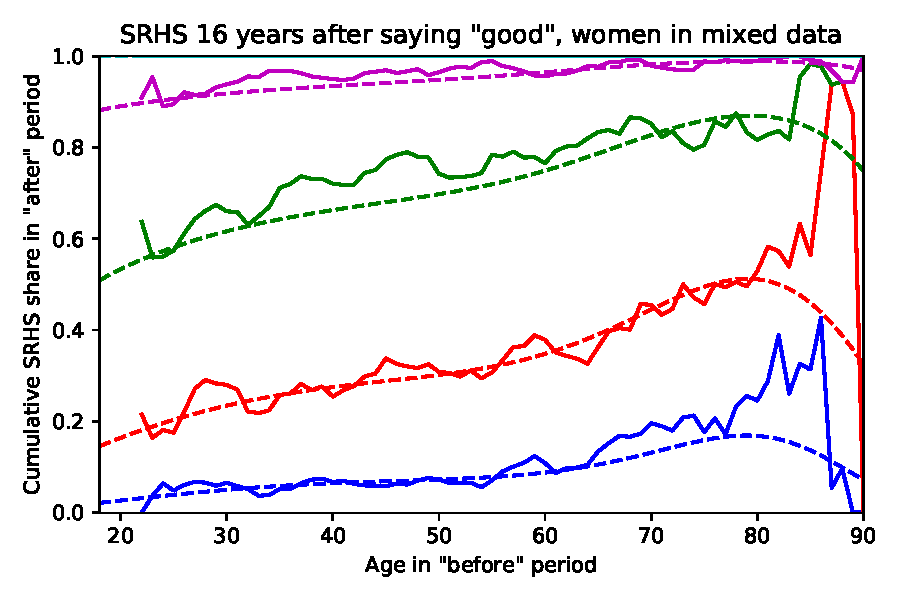
\includegraphics[width=\textwidth]{\FigsDir/CrossDataWomenTransH3T16modelNoLeg.pdf}
	    \caption{Sixteen years ahead}
    \end{subfigure}
    ~
    \begin{subfigure}[b]{0.45\textwidth}
	    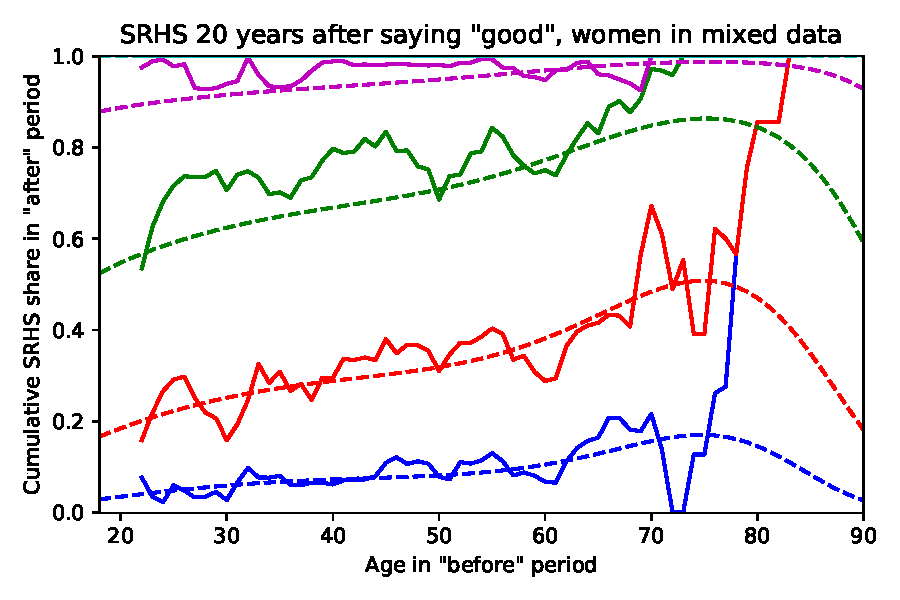
\includegraphics[width=\textwidth]{\FigsDir/CrossDataWomenTransH3T20modelNoLeg.pdf}
	    \caption{Twenty years ahead}
    \end{subfigure}

	\caption{Cumulative distribution of SRHS by age conditional on reporting ``good'' health in the baseline period in the mixed data (solid) vs estimated model (dashed)}\label{fig:ModelTransMixedGood}
\end{figure}
\thispagestyle{empty}


\begin{figure}[H]
	\centering
	\begin{subfigure}[b]{0.45\textwidth}
	    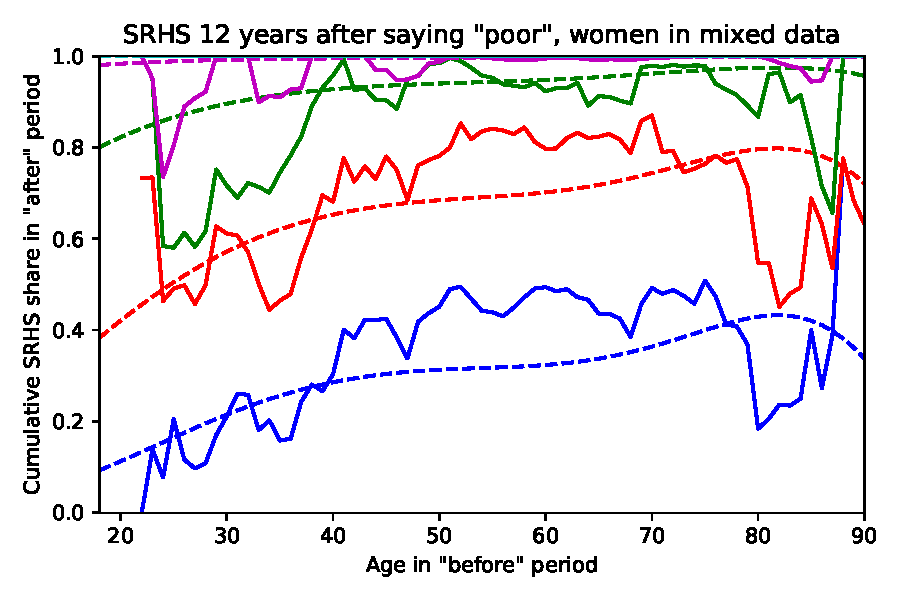
\includegraphics[width=\textwidth]{\FigsDir/CrossDataWomenTransH1T12modelNoLeg.pdf}
	    \caption{Poor health at baseline}\label{fig:Model12AheadPoor}
    \end{subfigure}
    ~
    \begin{subfigure}[b]{0.45\textwidth}
    	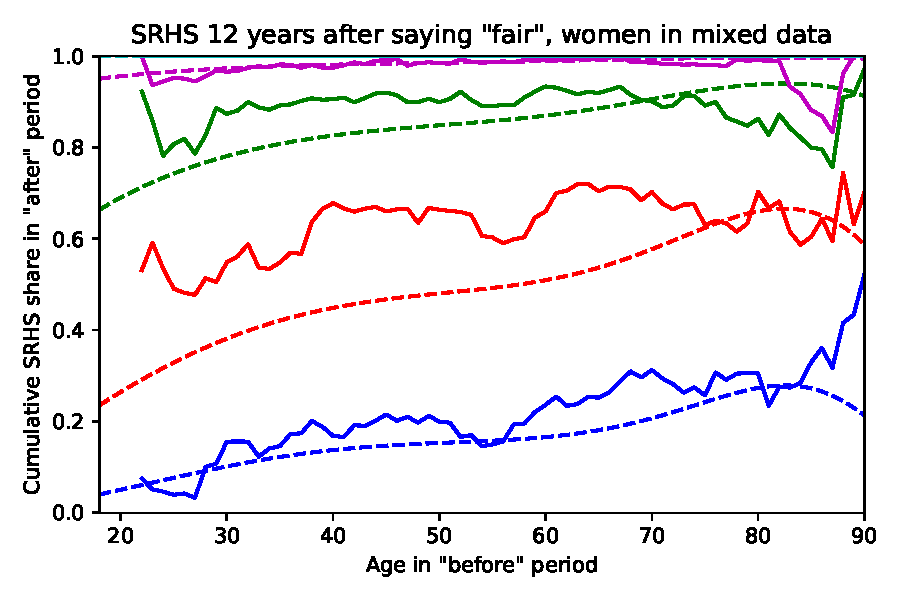
\includegraphics[width=\textwidth]{\FigsDir/CrossDataWomenTransH2T12modelNoLeg.pdf}
	    \caption{Fair health at baseline}\label{fig:Model12AheadFair}
    \end{subfigure}

    \begin{subfigure}[b]{0.45\textwidth}
    	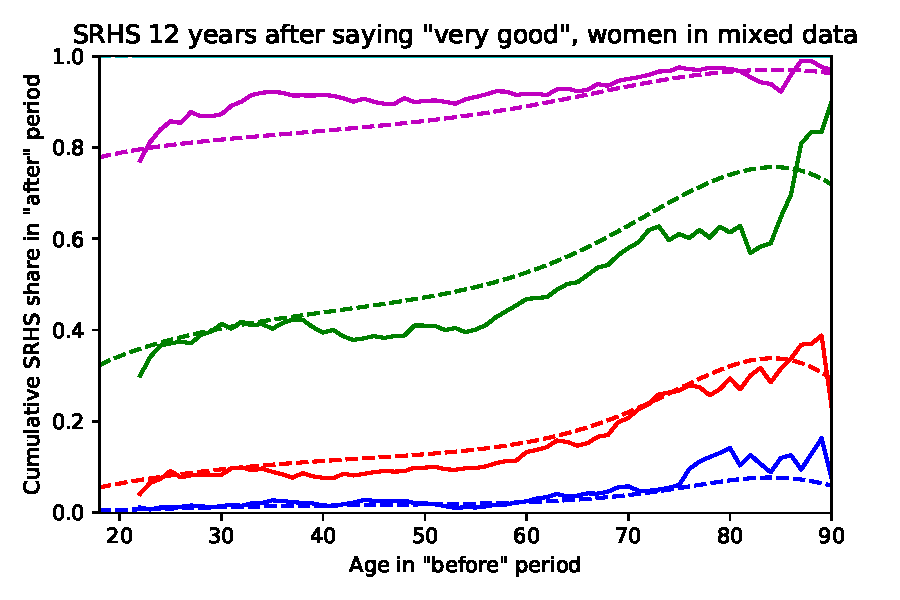
\includegraphics[width=\textwidth]{\FigsDir/CrossDataWomenTransH4T12modelNoLeg.pdf}
    	\caption{Very good health at baseline}\label{fig:Model12AheadVeryGood}
    \end{subfigure}
    ~
    \begin{subfigure}[b]{0.45\textwidth}
    	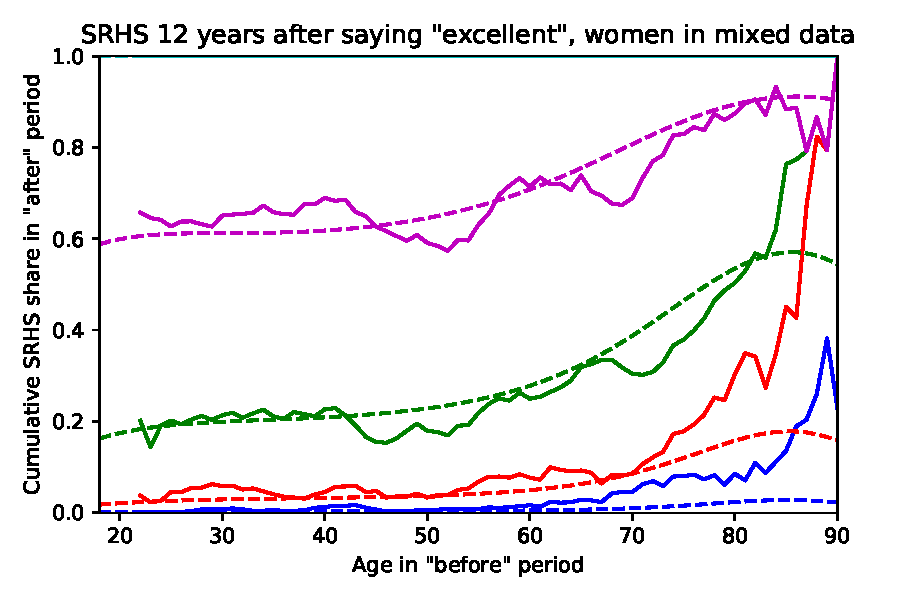
\includegraphics[width=\textwidth]{\FigsDir/CrossDataWomenTransH5T12modelNoLeg.pdf}
	    \caption{Excellent health at baseline}\label{fig:Model12AheadExcellent}
    \end{subfigure}	
	
	\begin{subfigure}[b]{0.45\textwidth}
		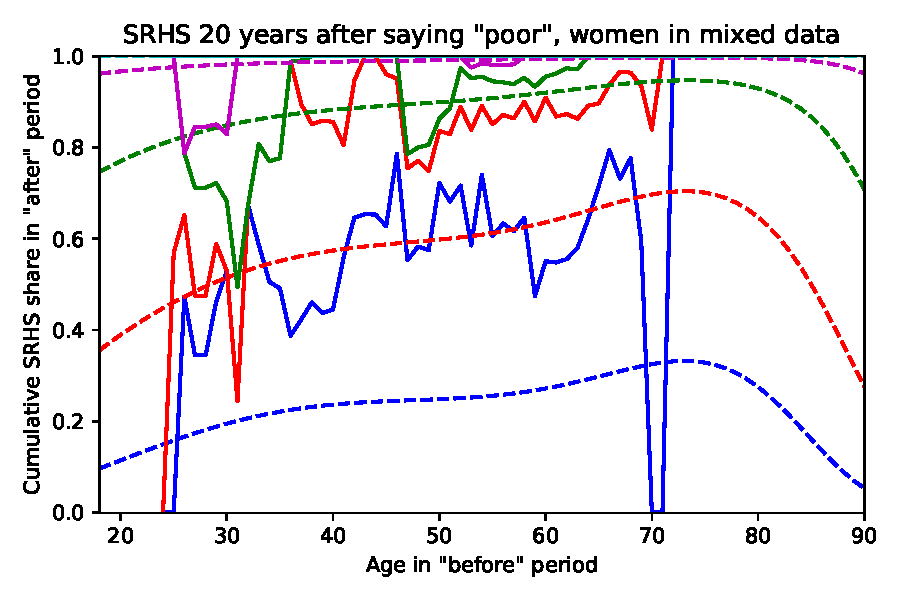
\includegraphics[width=\textwidth]{\FigsDir/CrossDataWomenTransH1T20modelNoLeg.pdf}
		\caption{Poor health at baseline}\label{fig:Model20AheadPoor}
	\end{subfigure}
	~
	\begin{subfigure}[b]{0.45\textwidth}
		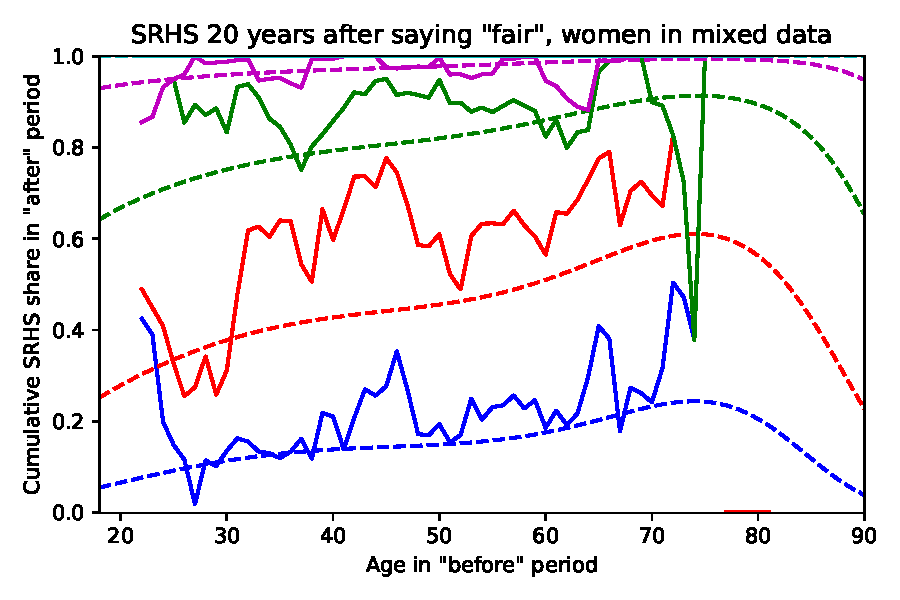
\includegraphics[width=\textwidth]{\FigsDir/CrossDataWomenTransH2T20modelNoLeg.pdf}
		\caption{Fair health at baseline}\label{fig:Model20AheadFair}
	\end{subfigure}
	
	\begin{subfigure}[b]{0.45\textwidth}
		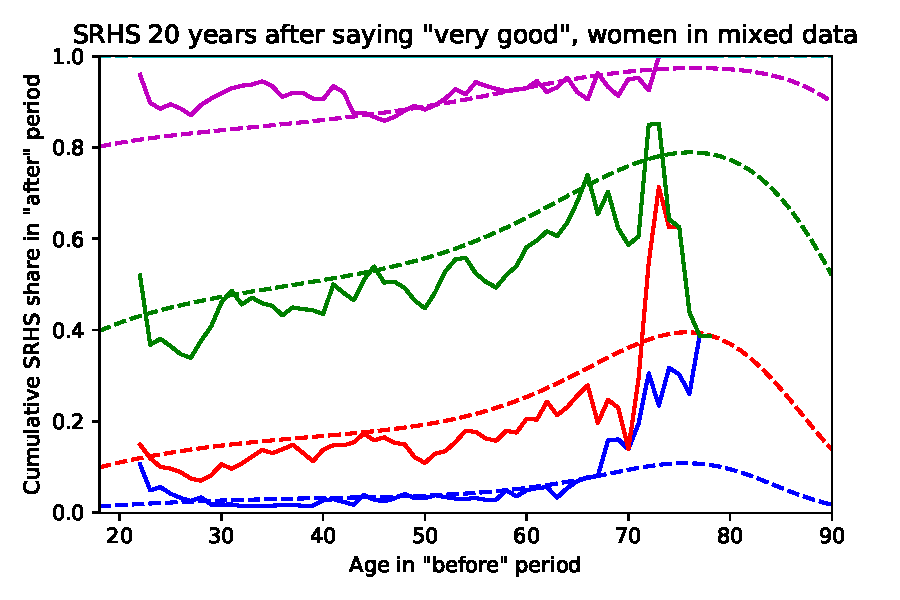
\includegraphics[width=\textwidth]{\FigsDir/CrossDataWomenTransH4T20modelNoLeg.pdf}
		\caption{Very good health at baseline}\label{fig:Model20AheadVeryGood}
	\end{subfigure}
	~
	\begin{subfigure}[b]{0.45\textwidth}
		\includegraphics[width=\textwidth]{\FigsDir/CrossDataWomenTransH5T20modelNoLeg.pdf}
		\caption{Excellent health at baseline}\label{fig:Model20AheadExcellent}
	\end{subfigure}
	\caption{Cumulative distribution of SRHS by age twelve and twenty years after the baseline period in the mixed data (solid) vs estimated model (dashed)}\label{fig:ModelTransMixed20Ahead}
\end{figure}
\thispagestyle{empty}

\newpage

\begin{figure}[H]
	\centering
	\begin{subfigure}[b]{0.48\textwidth}
		\includegraphics[width=\textwidth]{\FigsDir/CrossDataWomenDurDepT4B2G.pdf}
		\caption{Duration dependence of bad health}\label{fig:DurDepMixedWomenB2G}
	\end{subfigure}
	~
	\begin{subfigure}[b]{0.48\textwidth}
		\includegraphics[width=\textwidth]{\FigsDir/CrossDataWomenDurDepT4G2B.pdf}
		\caption{Duration dependence of good health}\label{fig:DurDepMixedomenG2B}
	\end{subfigure}
	\caption{Duration dependence of being ``healthy'' and ``unhealthy'' for women in mixed data (solid) vs estimated model (dashed).  A ``wave'' is the two years between data collection in the HRS and PSID; duration dependence cannot be observed in the MEPS-SAQ.}\label{fig:DurDepMixedWomen}
\end{figure}


\vspace{-0.5cm}
\begin{figure}[H]
	\centering
	\begin{subfigure}[b]{0.48\textwidth}
		\includegraphics[width=\textwidth]{\FigsDir/CorrelationWomen.pdf}
		\caption{Correlation coefficient for women}\label{fig:CorrWomen}
	\end{subfigure}
	~
	\begin{subfigure}[b]{0.48\textwidth}
		\includegraphics[width=\textwidth]{\FigsDir/CorrelationMen.pdf}
		\caption{Correlation coefficient for women}\label{fig:CorrMen}
	\end{subfigure}
	\caption{Estimated correlation coefficient on latent health across specifications.  MEPS specifications use six month periods, other specifications use one year periods.}\label{fig:Correlation}
\end{figure}

\vspace{-0.5cm}
\begin{figure}[H]
	\centering
	\begin{subfigure}[b]{0.48\textwidth}
		\includegraphics[width=\textwidth]{\FigsDir/CrossDataWomenChangeSRHS.pdf}
		\caption{Mixed data women}\label{fig:ChangeSRHSmixedWomen}
	\end{subfigure}
	~
	\begin{subfigure}[b]{0.48\textwidth}
		\includegraphics[width=\textwidth]{\FigsDir/CrossDataMenChangeSRHS.pdf}
		\caption{Mixed data men}\label{fig:ChangeSRHSmixedMen}
	\end{subfigure}
	\caption{Predicted probability of changing SRHS if asked twice in same survey}\label{fig:ChangeSRHSmixed}
\end{figure}


\newpage


\begin{figure}[H]
	\centering
	\begin{subfigure}[b]{0.48\textwidth}
		\includegraphics[width=\textwidth]{\FigsDir/CrossDataWomenSRHSfreqU25to34.pdf}
		\caption{``Unhealthy'' aged 25-34 at baseline}\label{fig:SRHSfreqU25to34}
	\end{subfigure}
	~
	\begin{subfigure}[b]{0.48\textwidth}
		\includegraphics[width=\textwidth]{\FigsDir/CrossDataWomenSRHSfreqH25to34.pdf}
		\caption{``Healthy'' aged 25-34 at baseline}\label{fig:SRHSfreqH25to34}
	\end{subfigure}

    \begin{subfigure}[b]{0.48\textwidth}
	    \includegraphics[width=\textwidth]{\FigsDir/CrossDataWomenSRHSfreqU45to54.pdf}
	    \caption{``Unhealthy'' aged 45-54 at baseline}\label{fig:SRHSfreqU45to54}
    \end{subfigure}
    ~
    \begin{subfigure}[b]{0.48\textwidth}
    	\includegraphics[width=\textwidth]{\FigsDir/CrossDataWomenSRHSfreqH45to54.pdf}
    	\caption{``Healthy'' aged 45-54 at baseline}\label{fig:SRHSfreqH45to54}
    \end{subfigure}


    \begin{subfigure}[b]{0.48\textwidth}
    	\includegraphics[width=\textwidth]{\FigsDir/CrossDataWomenSRHSfreqU65to74.pdf}
    	\caption{``Unhealthy'' aged 65-74 at baseline}\label{fig:SRHSfreqU65to74}
    \end{subfigure}
    ~
    \begin{subfigure}[b]{0.48\textwidth}
    	\includegraphics[width=\textwidth]{\FigsDir/CrossDataWomenSRHSfreqH65to74.pdf}
    	\caption{``Healthy'' aged 65-74 at baseline}\label{fig:SRHSfreqH65to74}
    \end{subfigure}
    \caption{Distribution of number of times reporting ``unhealthy'' SRHS by age and health over next six waves, mixed data vs estimated model.  Model fits distribution of frequency conditional on being ``healthy'' at baseline, but under-predicts probability of remaining ``unhealthy'' for next six waves after initially reporting being ``unhealthy''. }\label{fig:SRHSfreqMixedWomen}
\end{figure}


\newpage

\appendix

\section*{Literature Appendix}\label{app:LitQuotes}

This appendix provides a review of papers with a dynamic structural model that includes individual health as a state variable.  Its sole intent is to demonstrate that the ``naive dynamics'' of health described in Section \ref{sec:Intro} are employed nearly universally, often with little justification; relevant quotations are offered when possible.  I offer no discussion of the results or contributions of any paper.  Most of these works were published in the past decade or so, with some exceptions.

The first known (to me) dynamic structural model to include health as a state variable is found in \cite{RustPhelan97}, who use data from the Retirement History Survey, the precursor to the HRS, to explore how Social Security and Medicare rules motivate retirement behavior in an incomplete markets model.  They model the health state of a living individual as binary, with bad health indicated by answering affirmatively to either of, ``Do you have a health condition, physical handicap, or disability that limits how well you get around?'' or, ``Does your health limit the kind or amount of work or housework you can do?'' (p799-800).  The authors segregate ``the Markov transition matrix...\ representing individuals' \textit{one step ahead} beliefs'' into five components, one for each discrete state dimension.  These are each estimated separately in the first stage of their structural estimation; specifically, ``The marital status, health status, and mortality probabilities...\ were specified as binary logit probabilities and estimated via maximum likelihood.''  Although not stated directly, these quotes seem to imply that the estimation was conducted using only one-period transitions.

Two papers by the same coauthor team use HRS data to estimate transition probabilities of a binary health state.  \cite{BlauGilleskie06} estimate a structural model of joint decision-making by older married couples in which, ``[t]he transition probabilities are specified as first-order Markov logit processes.'' (p940)  In an early example of the now-standard approach, the authors use SRHS as the sole empirical measure of health, and combine the top three categories and bottom two categories to define their binary health state.  The authors write that, ``We take...\ health transitions from $t=$1-2, 2-3, and 3-4 as quantities to be explained by the model.  The model is estimated by maximum likelihood. The likelihood contribution is the product of [other outcome probabilities] and health transition probabilities.'' (p944)  The health process in \cite{BlauGilleskie08} is more complicated, but the same binary definition of health is used (p490).  They write, ``The health state in periods $t+1$ is determined by health in $t$, the medical care choices during period $t$, age, permanent unobserved heterogeneity, and an i.i.d.\ shock.'' (p482)  The transition probability is modeled as a logit with death as a third possible outcome, and the estimation is by maximum likelihood.  In both papers, an individual's reported health status is taken as given, so all transitions between binary states are treated as if they represent a true change in health.

\cite{Khwaja10} presents another dynamic discrete choice model estimated by maximum likelihood using HRS data.  Khwaja maintains all five categories of SRHS, and allows transition probabilities to be affected by the individual's discrete decisions over smoking, drinking, exercise, and medical utilization.  He specifies a multinomial logit form, estimating coefficients for five equations that determine the probability that an individual will be in \textit{at least} poor, fair, etc health; this is chosen for its additional flexibility relative to an ordered probit or logit (p133).  As above, SRHS is treated as a true representation of health, and there is no reference to the model's ability to fit transitions more than one period ahead.

Three papers by a famous research team all employ the same approach to modeling health dynamics.  \cite{French11} use HRS data to estimate transition probabilities of their binary health state (using the standard SRHS partition).  They do not specify an estimation method, but the text hints that it must be fairly simple: ``In the first step, we estimate or calibrate parameters that can be cleanly identified without explicitly using our model.  For example, we estimate mortality rates and health transitions straight from demographic data.'' (p702)  No other mention of the health process is made other than a single sentence: ``Health status and mortality both depend on previous health status interacted with an age polynomial.'' (p709)  Contemporaneous work in \cite{DeNardi10} also uses exogenous transitions between binary health states, and the authors specify that they, ``estimate the probability of death and bad health as logistic functions of a cubic in age, sex, sex interacted with age, previous health status, health status interacted with age, a quadratic in permanent income rank, and permanent income rank interacted with age.''  Later, \cite{DeNardi16} add a third discrete health state, for individuals in a nursing home; exogenous transition probabilities ``depend on previous health, sex, permanent income, and age.'' (p3492)  Like \cite{Khwaja10}, they ``estimate health transitions and mortality rates simultaneously by fitting the transitions observed in the HRS to a multinomial logit model.'' (p3497)

\cite{Pashchenko13} estimate a rich structural model to analyze the welfare effects of health insurance reform measures styled after the Affordable Care Act.  They model a binary health state that is fully coincident with medical expenses: ``We categorize individuals into two groups according to their medical expenses.  Individuals with low medical expenses ($x_t \leq \bar{x}_t$ are referred to as `healthy' or `people in good health', while individuals with high medical expenses ($x_t > \bar{x}_t$) are referred to as `unhealthy' or `people in bad health'." (p385)  They specify five medical expense ``bins'' for each age, with the lower three bins corresponding to ``good'' health.  Concerning the Markov transition probabilities among the bins, they write, ``To construct the transition matrix we measure the fraction of people who move from one bin to another between two consecutive years separately for people of working age (25-64) and for retirees (older than 65).'' (p394) They thus explicitly specify using a simple frequency count on observed one-period transitions.

\cite{Ferreira17} likewise investigate the effects of ACA-style reforms on consumer welfare, with a particular focus on medical cost reductions.  They model individual health as binary and ``evolving according to a first-order Markov process.'' (p131)  The standard partition of the SRHS question on the MEPS is used to define the health state.  Authors specify that they, ``estimated the transition probabilities using the logit method.  We regressed next period's health status on a constant, age, age squared, age cubic, education level, current health status, and age times current health status.''  Again, only one-period transitions are used to estimate the dynamics of health.

\cite{LowPistaferri15} do not use SRHS as their health state, but instead model transitions among three levels of work limitations: none, moderate, and severe.  They construct this measure using a series of questions in the PSID that ask the respondent whether they have any condition that limits the type or amount of work they can do, then probes any positive answer for the extent (p2999).  Transition probabilities among the three health states are assumed to be Markov(1), and the authors write that, ``some parameters are estimated outside the structure of the model.  For some parameters, this is because no structure is needed: disability risk can be estimated directly from transitions between disability states because of the exogeneity assumption.''  While questions about work limitations might be subject to \textit{less} reporting error than the more ambiguous SRHS question, some observed transitions are still likely spurious, adversely affecting the model's ability to fit disability transitions more than one wave ahead.

In very recently published work, \cite{Aizawa19} examines how workers sort into jobs that do or don't offer employer-sponsored health insurance, and how this is affected by an ACA-style employer mandate.  He specifies health as binary, with transition probabilities determined by a logistic function of health, age, and other current period variables (p1409).  He uses the standard partition of SRHS categories to separate the ``healthy'' from the ``unhealthy'', utilizing data from both the MEPS and the Survey of Income and Program Participation (p1423).  The model is estimated by the simulated method of moments; parameters governing health transition probabilities are identified by three kinds of moments:\footnote{All moments are also conditional on the individual's age.} ``(a) health status conditional on employment and health insurance status; (b) annual health transition conditional on health; [and] (c) annual health transition conditional on health and health insurance status.'' (p1427) In this way, only one-period SRHS transitions are used to estimate the dynamics of health, causing the model to badly match longer run transitions.

In a related paper, \cite{AizawaFang18} model two-dimensional binary health, with one component observed by the econometrician and the other unobserved; authors also use the SRHS question in the MEPS and SIPP (with the standard partition) as their empirical measure of (observed) health.  The observed component of the health state follows a Markov process, with probabilities varying by demographic type and insurance status (pp7-8); the unobserved component represents permanent heterogeneity and is time invariant (p22).  Transition probabilities are estimated by maximum likelihood, accounting for the fact that observations of SRHS are annual but the model is calibrated at the triannual frequency by considering all intermediate, unobserved paths of SRHS.  However, each $t$ to $t+3$ transition is treated as an independent contribution to the likelihood function.  The estimated transition probabilities will thus distribute observed annual changes over three four-month periods, but will still overestimate the true volatility of health.

I know of only two dynamic structural models of health that do \textit{not} use a discrete representation with naive dynamics.  \cite{JungTran16} take the classic Grossman health capital model seriously, modeling health as a continuous variable with stochastic depreciation.  They use the SF-12v2 physical health index in the MEPS as their empirical measure of health, mapped to a grid with 15 nodes (p142), and use frequency counts to calibrate the likelihood of health shocks of various magnitudes.  Using data from the HRS, \cite{White18} constructs a continuous measure of health by estimating an ordered probit of SRHS on a long list of specific health outcomes, then projecting fitted values onto the unit interval.  The health transition process is estimated by SMM in the main estimation step, fitting age-profiles of mean health by income group and initial health status.  Some evidence of measurement error in the constructed health index is found, but an order of magnitude smaller than estimated in this paper-- a standard deviation about one-fifth that of a one-period health shock, rather than twice as great as with SRHS.

\end{document}